\documentclass[enabledeprecatedfontcommands,fontsize=11pt,paper=a4,twoside]{scrartcl}

\newcommand*{\red}{\textcolor{red}}
\newcommand*{\blue}{\textcolor{blue}}
\newcommand*{\bbe}{\textcolor{bbe}}

\newcommand{\grad}{\ensuremath{^{\circ}} }
\renewcommand{\strut}{\vrule width 0pt height5mm depth2mm}

\usepackage[utf8]{inputenc}
\usepackage[T1]{fontenc}
\usepackage[final]{pdfpages}
% obere Seitenränder gestalten können
\usepackage{fancyhdr}
\usepackage{moreverb}
% Graphiken als jpg, png etc. einbinden können
\usepackage{graphicx}
\usepackage{stmaryrd}
% Floats Objekte mit [H] festsetzen
\usepackage{float}
% setzt URL's schön mit \url{http://bla.laber.com/~mypage}
\usepackage{url}
% Externe PDF's einbinden können
\usepackage{pdflscape}
% Verweise innerhalb des Dokuments schick mit " ... auf Seite ... "
% automatisch versehen. Dazu \vref{labelname} benutzen
\usepackage[ngerman]{varioref}
\usepackage[ngerman]{babel}
\usepackage{ngerman}
% Bibliographie
\usepackage{bibgerm}
\usepackage{svg}
% Tabellen
\usepackage{tabularx}
\usepackage{supertabular}
\usepackage[colorlinks=true, pdfstartview=FitV, linkcolor=blue,
            citecolor=blue, urlcolor=blue, hyperfigures=true,
            pdftex=true]{hyperref}
\usepackage{bookmark}



\newcounter{one}
\newcounter{two}[one]
\newcounter{three}[two]

\newcommand{\tone}{0\theone}
\newcommand{\ttwo}{0\thetwo}
\newcommand{\tthree}{0\thetree}
\newcommand{\one}{\stepcounter{one}0\theone}
\newcommand{\two}{\stepcounter{two}0\thetwo}
\newcommand{\three}{\stepcounter{three}0\thethree}
\newcommand\s{\rule{0pt}{4ex}}        
\newcommand{\cb}[1]{{\textcolor{blue}{#1}}}
\newcommand*{\hint}{\paragraph{\textcolor{blue}{Hinweise}}}
\newcommand*{\condition}{\paragraph{Voraussetzung}$\;$ \vspace{0.2cm}\\}
\newcommand*{\actions}{\paragraph{Vorgehen} $\;$\vspace{0.2cm}\\}
\newcommand*{\action}{\paragraph{Vorgehen}}
\newcommand*{\hdot}{\\ \hdashline[1pt/5pt]}
\newcommand*{\hdo}{.............}
\newcommand*{\aOne}{\textcolor{bbe}{Alternative 1:}}
\newcommand*{\aTwo}{\textcolor{bbe}{Alternative 2:}}
\newcommand*{\aThree}{\textcolor{bbe}{Alternative 3:}}
\newcommand*{\aFour}{\textcolor{bbe}{Alternative 4:}}



\usepackage{geometry}
\usepackage{hyperref}
\usepackage{pdfpages} 
\usepackage{colortbl}
%\usepackage{graphicx}   
%\usepackage[utf8x]{inputenc}
\usepackage{fmtcount}
\usepackage[ngerman]{babel}
\usepackage{booktabs}
\usepackage{fancyhdr}
\usepackage[T1]{fontenc}
\usepackage{nameref}
\usepackage{graphicx}
\usepackage{subfigure}


\pagestyle{fancy}
\fancyhf{}

%

%

%

%

\definecolor{dartmouthgreen}{rgb}{0.05, 0.5, 0.06}
\definecolor{color}{rgb}{0.67, 0.88, 0.69}
\definecolor{todo}{rgb}{1.0, 0.41, 0.71}
\definecolor{sort}{rgb}{0.45, 0.76, 0.98}
\definecolor{prob}{rgb}{0.74, 0.83, 0.9}
\definecolor{anw}{rgb}{0.94, 0.86, 0.51}
\definecolor{ghostwhite}{rgb}{0.97, 0.97, 1.0}
\definecolor{glaucous}{rgb}{0.38, 0.51, 0.71}
\definecolor{bbe}{rgb}{0.13, 0.67, 0.8}
\usepackage{amsmath}
\usepackage{tabularx}
\usepackage{setspace} 
\hypersetup{
	colorlinks = true,
	linkbordercolor = {white},
	linkcolor=dartmouthgreen,          % color of internal links (change box color with linkbordercolor)
	citecolor=red,        % color of links to bibliography
	filecolor=magenta,      % color of file links
	urlcolor=cyan 
}
\usepackage{geometry}
\geometry{
	a4paper,
	left=20mm,
	right=20mm,
	top=2cm,
	bottom=4cm,
	footskip=4cm
}


\addtolength{\headwidth}{20mm}
\addtolength{\headheight}{2\baselineskip}
\addtolength{\headheight}{0.61pt}


\renewcommand{\headrulewidth}{0pt}
\renewcommand{\headrule}{\vbox to 0pt{\rule{\headwidth}{0.2pt}}}
\setlength{\headsep}{30pt}


\let\tempone\itemize
\let\temptwo\enditemize
\renewenvironment{itemize}{\tempone\addtolength{\itemsep}{-10.0pt}}{\temptwo}

\let\origenumerate\enumerate
\let\origendenumerate\endenumerate
\renewenvironment{enumerate}{\origenumerate \addtolength{\itemsep}{-10.0pt}}{\origendenumerate}

%\addtolength{\itemsep}{-10.0pt}
%\setitemize{itemsep=-10.0pt}
%\setenumerate{itemsep=-10.0pt}

\hyphenation{Arbeits-paket}

% Damit Latex nicht zu lange Zeilen produziert:
%\sloppy
%Uneinheitlicher unterer Seitenrand:
%\raggedbottom

% Kein Erstzeileneinzug beim Absatzanfang
% Sieht aber nur gut aus, wenn man zwischen Absätzen viel Platz einbaut
%\setlength{\parindent}{0ex}

% Abstand zwischen zwei Absätzen
%\setlength{\parskip}{1ex}

% Seitenränder für Korrekturen verändern
%\addtolength{\evensidemargin}{-1cm}
%\addtolength{\oddsidemargin}{1cm}

%\bibliographystyle{gerapali}

% Lustige Header auf den Seiten
  \pagestyle{fancy}
  \setlength{\headheight}{70.55003pt}
  \fancyhead{}
  \fancyhead[LO,RE]{Software--Projekt 2\\ WiSe 2018/2019
  \\Architekturbeschreibung}
  \fancyhead[LE,RO]{Seite \thepage\\\slshape \leftmark\\\slshape \rightmark}

%
% Und jetzt geht das Dokument los....
%

\begin{document}

% Lustige Header nur auf dieser Seite
  \thispagestyle{fancy}
  \fancyhead[LO,RE]{ }
  \fancyhead[LE,RO]{Universität Bremen\\FB 3 -- Informatik\\
  Prof. Dr. Rainer Koschke \\TutorIn: Marcel Steinbeck}
  \fancyfoot[C]{}

% Start Titelseite
  \vspace{3cm}

  \begin{minipage}[H]{\textwidth}
  \begin{center}
  \bf
  \Large
  Software--Projekt 2 WiSe 2018/2019\\
  \smallskip
  \small
  VAK 03-BA-901.02\\
  \vspace{3cm}
  \end{center}
  \end{minipage}
  \begin{minipage}[H]{\textwidth}
  \begin{center}
  \vspace{1cm}
  \bf
  \Large Benutzerhandbuch\\
  \vspace{2cm}
  
\includegraphics[width=3.0in]{logo_graphit.png}

  
  \end{center}
 
  \end{minipage}
  \vfill
  \begin{minipage}[H]{\textwidth}
  \begin{center}
  \sf
  \begin{tabular}{lr}
  Anthony Mendil & antmen@tzi.de \\
  Bastian Rexhäuser & brexhaeu@tzi.de\\
  Clement Phung & clement1@tzi.de \\
  Jacky Philipp Mach & machja@tzi.de \\
  Jonah Jaeger & jjaeger@tzi.de \\
  Nina Unterberg & nin\_unt@tzi.de \\
  \end{tabular}
  \\ ~
  \vspace{2cm}
  \\
  \it Abgabe: 10. März 2019 --- Version 1.0\\ ~
  \end{center}
  \end{minipage}

% Ende Titelseite

% Start Leerseite

\newpage

  \thispagestyle{fancy}
  \fancyhead{}
  \fancyhead[LO,RE]{Software--Projekt \\  2018/2019
  \\Benutzerhandbuch}
  
  \fancyhead[LE,RO]{Seite \thepage\\\slshape \leftmark\\~}
  \fancyfoot{}
  \renewcommand{\headrulewidth}{0.4pt}
  \tableofcontents

\newpage

  \fancyhead[LE,RO]{Seite \thepage\\\slshape \leftmark\\\slshape \rightmark}

%%%%%%%%%%%%%%%%%%%%%%%%%%%%%%%%%%%%%%%%%%%%%%%%%%%%%%%%%%%%%%%%%%%%%%%%
%%%%%%%%%%%%%%%%%%%%%%%%%%%%%%%%%%%%%%%%%%%%%%%%%%%%%%%%%%%%%%%%%%%%%%
\section*{Vorwort}
Mit diesem Handbuch wird die Bedienung der Software \textbf{GraphIT} beschrieben. Diese Anwendung wurde im Rahmen des Moduls \glqq{Softwareprojekt 2}\grqq im Wintersemester 2018/19 entwickelt und ist zur Erstellung, Editierung und Visualisierung von Wirkungsdiagrammen für den Syndromansatz entworfen worden. \\
Eine Nutzung des Programmes für Zwecke, die von dem angedachten Einsatzbereich abweicht ist möglich. Allerdings wird in diesem Dokument nicht weiter auf eine solche Nutzung eingegangen. Bei dieser Nutzung, die nicht dem angedachten Einsatz entspricht, ist ferner zu berücksichtigen, dass eventuell gewisse Funktionen wünschenswert wären, die aufgrund der Anforderungen jedoch bewusst nicht eingebaut wurden. Insbesondere sind hier die Regeln zu beachten, die für die Erstellung von Wirkungszusammenhängen gemäß des Syndromansatzes gelten. \\
Bei der vorliegenden Software handelt es sich um eine Neu-Entwicklung. Somit existieren keinerlei Vorversionen, mit denen der Funktionsumfang oder die Bedienung der Software in diesem Dokument verglichen werden könnte. 

%%%%%%%%%%%%%%%%%%%%%%%%%%%%%%%%%%%%%%%%%%%%%%%%%%%%%%%%%%%%%%%%%%%%%%%%
%%%%%%%%%%%%%%%%%%%%%%%%%%%%%%%%%%%%%%%%%%%%%%%%%%%%%%%%%%%%%%%%%%%%%%
\section{Einführung}
\subsection{Adressierte Leser}
Dieses Handbuch richtet sich an alle Nutzer, die \textbf{GraphIt} für ihren bestimmungsgemäßen Einsatz verwenden möchten. Dieser umfasst die Erstellung, Bearbeitung und Auswertung von Wirkungszusammenhängen gemäß des Syndromansatzes. Die Software ist sowohl für Anfänger geeignet, die noch nie oder nur sehr selten mit einem vergleichbaren Programm gearbeitet haben, als auch für Fortgeschrittene und Experten, die über mehr Erfahrung in der Bedienung ähnlicher Software verfügen. \\
Von dem Adressatenkreis des vorliegenden Dokuments wird die Kenntnis der Terminologie des Syndromansatzes erwartet.  
\subsection{Verwandte Dokumente}
Neben dem Benutzerhandbuch der Software \textbf{GraphIt}, existiert ebenfalls ein Testprotokoll, welches die Entwickler erstellt haben, um die Korrektheit der Software zu garantieren. Außerdem eine Architekturbeschreibung die detaillierteren Einblick in die Architektur der Software gewährt. 
\subsection{Konventionen}
\begin{itemize}
	\item Wenn im Verlaufe des Dokumentes von einem Graphen die Rede ist, wird sich auf ein Wirkungsdiagramm  gemäß des Syndromansatzes bezogen.
\end{itemize}

\subsection{Informationen über die Verwendung des Dokuments}

\begin{itemize}
	\item Alle eingebundenen Screenshots in das Dokument wurden auf einem Computer mit Windows 10 Betriebssystem aufgenommen. Wenn ihre Darstellung der Software leicht von den gerade erwähnten Screenshots abweicht, bitten wir dies zu entschuldigen.
	\item Um die Software \textbf{GraphIt} am Besten verstehen und anwenden zu können, empfehlen wir das Dokument von Anfang bis Ende durchzuarbeiten, da sich manche Einträge auf vorherige beziehen. 
\end{itemize}



%%%%%%%%%%%%%%%%%%%%%%%%%%%%%%%%%%%%%%%%%%%%%%%%%%%%%%%%%%%%%%%%%%%%%%
\newpage
\section{Installation und Starten des Programms} \label{sec:installation}

\subsection{Installationsvoraussetzungen}
\subsubsection{Java 8}
\red{TODO}

\subsection{Installationsanweisungen}
\begin{itemize}
	\item \red{TODO}
\end{itemize}
\subsection{Starten des Programms}
\red{TODO}

\newpage	
%%%%%%%%%%%%%%%%%%%%%%%%%%%%%%%%%%%%%%%%%%%%%%%%%%%%%%%%%%%%%%%%%%%%%		
\section{Benutzeroberfläche}
\subsection{Tasten-/ Mausbelegungen}

\begin{tabular} {|p{8cm}|p{8cm}|}
	\hline
	\rowcolor{glaucous}\multicolumn{2}{|l|} {\parbox{16cm}{\textbf{\textcolor{ghostwhite}{Maus-/ Tastenbelegungen}}} } \\ \hline\hline 	
	Drucken	& Ctrl + P \\ \hline
	Neue Datei	& Ctrl + N \\ \hline
	GXL importieren	& Ctrl + Shift + I \\ \hline
	Speichern unter	&	Ctrl + S \\ \hline
	\red{TODO} & \\ \hline
\end{tabular}

 
\subsection{Übersicht}
1\hdo..Sphäre hinzufügen -Button \\
2\hdo..Auswahl -Button \\
3\hdo..Sphäre entfernen \\
4\hdo..Sphäre vergrößern \\
5\hdo..Sphäre verkleinern \\
6\hdo..Sphäre Füllfarbe verändern  \\
7\hdo..Sphäre Schriftart verändern  \\
8\hdo..Sphäre Schriftgröße verändern \\
9\hdo..Sphäre layouten \\
10\hdo  Symptom hinzufügen \\
11\hdo  Symptom entfernen \\
12\hdo  Symptom vergrößern \\
13\hdo  Symptom verkleinern \\
14\hdo  Symptom Füllfarbe verändern \\
15\hdo  Symptom Randfarbe verändern \\
16\hdo  Symptom Form verändern \\
17\hdo  Symptome layouten \\
18\hdo  Symptome Schriftart verändern \\
19\hdo  Symptome Schriftgröße verändern \\
20\hdo  Ankerpunkte einblenden \\
21\hdo  Relation entfernen \\
22\hdo  Relation Ankerpunkte entfernen \\
23\hdo  Relation Farbe verändern \\
24\hdo  Relation Kantenart  verändern \\
25\hdo  Relation Typ verändern \\
26\hdo  nach Relationstyp filtern \\
27\hdo  nach Regex filtern \\
28\hdo  Übersichtsleiste \\
29\hdo  Zoom Fenster  \\
30\hdo  Vorlage\\
31\hdo  Maximale Anzahl von Graph- Elementen\\
34\hdo  Relationen erlauben \\
35\hdo Sperrende Elemente auswählen \\
36\hdo Zoom-leiste \\
37\hdo aktuelle Mausposition \\
38\hdo Bearbeiter Modus\\
39\hdo Ersteller Modus\\
40\hdo Analyse Modus\\
41\hdo Undo/ rückgängig machen\\
42\hdo redo/ wiederholen\\
43\hdo gehighlighte Elemente ein-/ausblenden\\
44\hdo Element highlighten\\
45\hdo Element aus dem Highlight entfernen\\
46\hdo Elemente ein-/ausblenden\\
47\hdo Element zum Fadeout hinzufügen\\
48\hdo Element aus Fadeout entfernen\\
49\hdo Neue Datei hinzufügen\\
50\hdo Datei öffnen\\
51\hdo GXL importieren\\
52\hdo Speichern unter\\
53\hdo Exportieren als PDF/ GXL/ Verlaufsprotokoll\\
54\hdo Drucken\\
55\hdo Sprache Benutzeroberfläche\\
56\hdo Sprache des Graphen\\
57\hdo Dokumentation\\
58\hdo über uns \\
59\hdo Graphmaße\\
60\hdo Vorgänger/ Nachfolger\\
61\hdo Anzahl\\
62\hdo Kürzester Weg/ alle Wege\\
63\hdo Analyse-Optionen: Pfeilketten, Konvergente/ Divergente Verzweigungen, Verzweigungen,\\ 		
\hspace*{1.7cm} Zyklen\\
64\hdo Verlaufsübersicht\\
65\hdo Liste der Logs synchronisieren\\
66\hdo Filtern nach dem Verlaufstyp\\

\red{TODO - Screenshots bearbeiten}

\begin{landscape}
	\begin{figure}
		\centering
		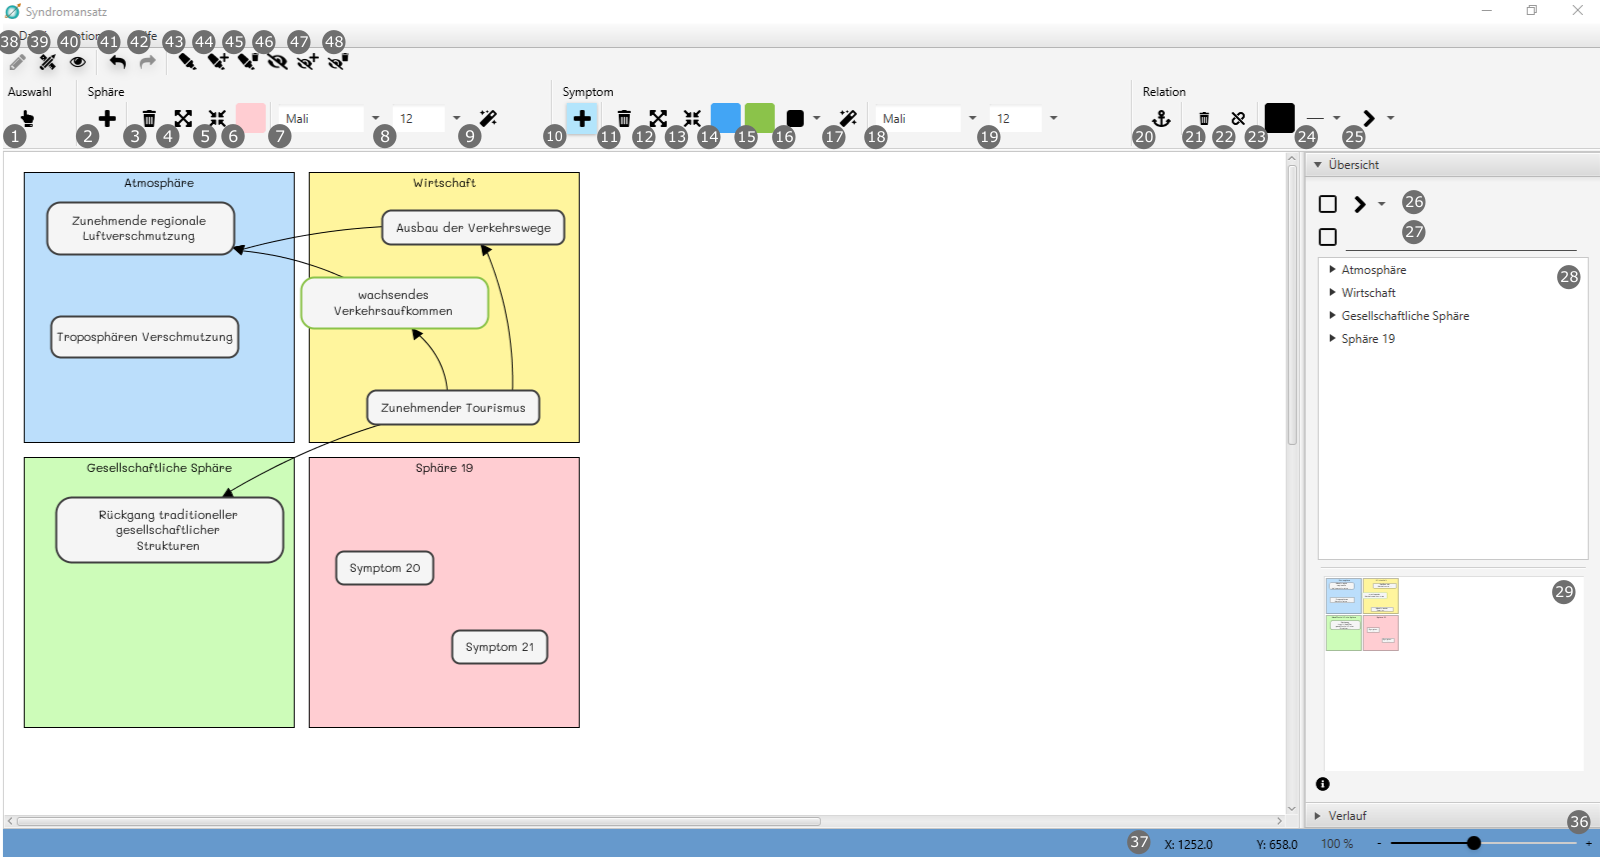
\includegraphics[width=22cm]{overview.png}
		\caption{Übersicht über den Ersteller Modus}
		\label{fig:label}
	\end{figure}
\end{landscape}
\begin{landscape}
	\begin{figure}
		\centering
		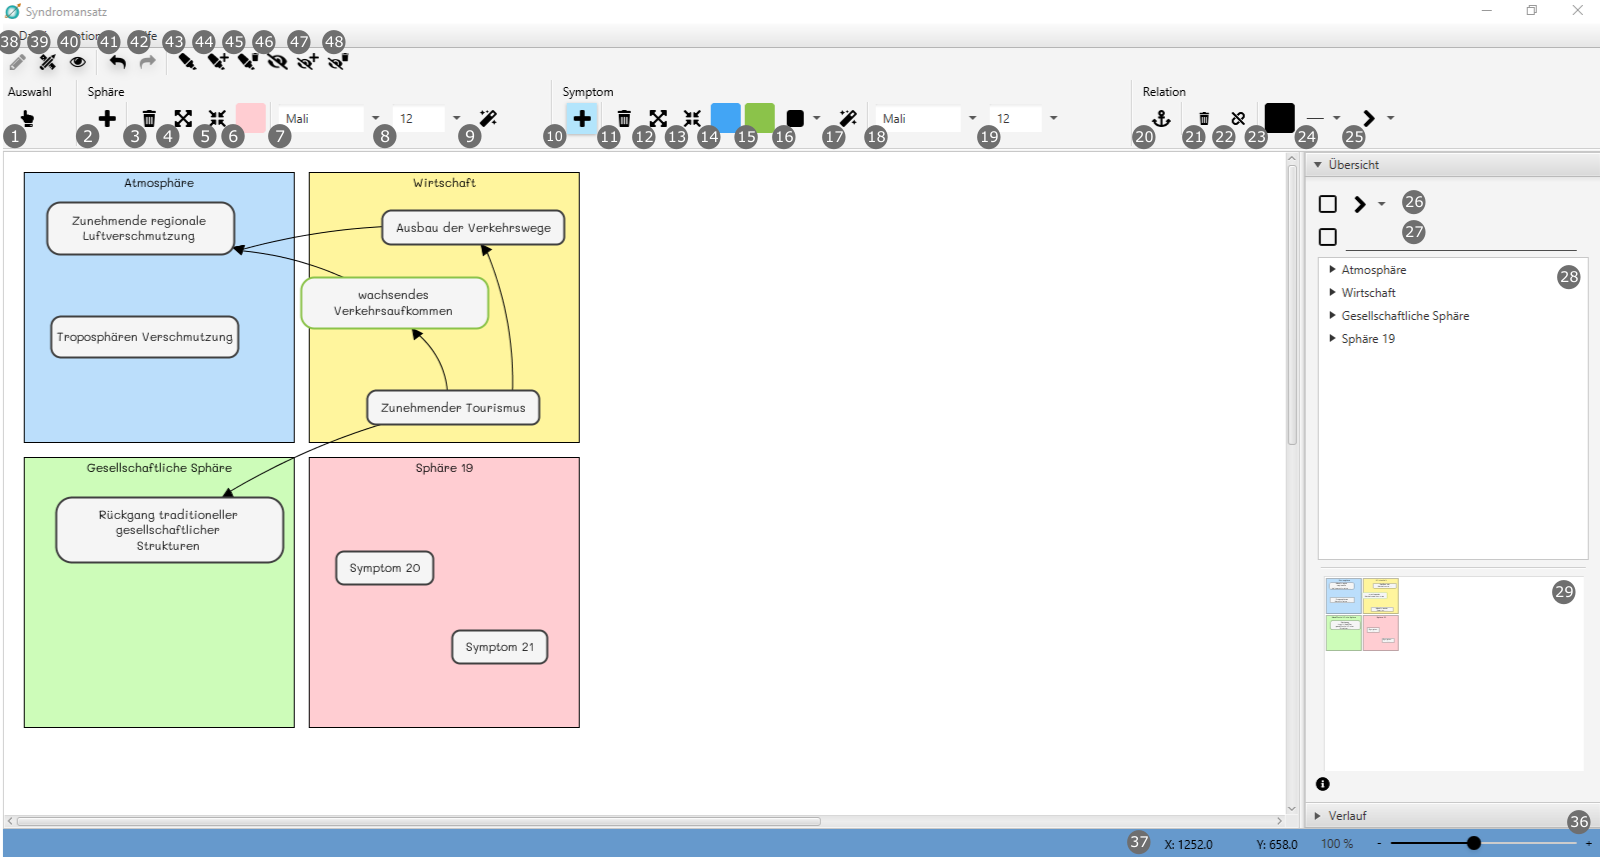
\includegraphics[width=22cm]{overview.png}
		\caption{Übersicht über den Analyse Modus}
		\label{fig:label}
	\end{figure}
\end{landscape}




\newpage	
%%%%%%%%%%%%%%%%%%%%%%%%%%%%%%%%%%%%%%%%%%%%%%%%%%%%%%%%%%%%%%%%%%%%%%	
\section{Übersicht} \label{sec:uebersicht}
\subsection{Ersteller Modus}
Im \texttt{Ersteller Modus} kann der Benutzer einen Syndromansatz erstellen und editieren. Im Unterschied zu dem \nameref{sec:editor} kann der Benutzer Vorlageregel für den aktuellen Syndromansatz hinterlegen. Diese werden erst auf dem Graphen im \nameref{sec:editor} angewandt. 


\subsubsection{Relevante Kapitel}
\begin{itemize}
	\item \nameref{pick}
	\item \nameref{edit}
	\item \nameref{sphere}	
	\item \nameref{symptom}	
	\item \nameref{relations}	
	\item \nameref{template}
	\item \nameref{overwiew}
	\item \nameref{zoom}
	\item \nameref{export}
	\item \nameref{import}
	\item \nameref{print}
	\item \nameref{dialog}
	\item \nameref{fehlermeldungen}
	\item \nameref{settings}	
\end{itemize}
\subsection{Bearbeiter Modus} \label{sec:editor}
Im \texttt{Bearbeiter Modus} kann der Benutzer einen Syndromansatz erstellen und bearbeiten. Die Bearbeitung des Graphen folgt den hinterlegten Vorlageregeln. Alle Aktionen auf dem Graph werden geloggt, d.h. ein Verlaufsprotokoll erstellt, welches ebenfalls einsehbar und exportierbar/ importierbar ist. 
\subsubsection{Relevante Kapitel}
\begin{itemize}
	\item \nameref{pick}
	\item \nameref{edit}
	\item \nameref{sphere}	
	\item \nameref{symptom}	
	\item \nameref{relations}	
	\item \nameref{logs}
	\item \nameref{overwiew}
	\item \nameref{zoom}
	\item \nameref{export}
	\item \nameref{import}
	\item \nameref{print}
	\item \nameref{dialog}
	\item \nameref{fehlermeldungen}
	\item \nameref{settings}	
\end{itemize}
\subsection{Analyse Modus}
Im \texttt{Analyse Modus} kann ein Syndromansatz analysiert und ausgewertet werden. In diesem Modus ist keine Bearbeitung des Graphen möglich. \\
Die Analyse umfasst z.B. die Lokalisierung von Pfeilketten oder die Berechnung des kürzesten Weges zwischen 2 Symptomen. \\
Die Auswertung der Nutzerinteraktionen ist ebenfalls möglich. Diese können vom Benutzer gefiltert und angezeigt werden. 
\subsubsection{Relevante Kapitel}
\begin{itemize}
	\item \nameref{pick}	
	\item \nameref{logs}
	\item \nameref{overwiew}
	\item \nameref{zoom}
	\item \nameref{export}
	\item \nameref{import}
	\item \nameref{print}
	\item \nameref{dialog}
	\item \nameref{fehlermeldungen}
	\item \nameref{settings}	
	\item \nameref{analyse}
\end{itemize}

%%%%%%%%%%%%%%%%%%%%%%%%%%%%%%%%%%%%%%%%%%%%%%%%%%%%%%%%%%%%%%%%%%%%%%%

\newpage
\section{Instruktionen zur Nutzung des Programms} \label{sec:nutzung}

		\subsection{Auswahl von Graphelementen} \label{pick}
	\subsubsection{Eines Elements}
	\condition
	Es muss ein Syndrom mit mindestens einem Element (eine Sphäre/ ein Symptom/ eine Relation), welches ausgewählt werden soll, existieren. 
	\actions
	\aOne 
	\begin{enumerate}
		\item In der Menüleiste den Button \textit{Auswahl} durch einen Links-Klick aktivieren. 
		\item Den Cursor auf das Element bewegen und die linke Maustaste klicken. 
	\end{enumerate}
	\aTwo
	\begin{enumerate}
		\item In der Übersichtleiste das auszuwählende Element durch einen Links-Klick auswählen. 
	\end{enumerate}
	\hint
	\begin{itemize}
		\item Eine Relation kann manchmal etwas schwierig auszuwählen sein, da die Kanten vergleichsweise relativ dünn sind. 
		\item Die Nutzung der eben angesprochenen Übersichtsleiste wird in einem folgenden Unterkapitel (\ref{overwiew}) noch genauer beschrieben.
		\item Ausgewählte Elemente werden in der Visualisierung durch einen dickere Umrandung hervorgehoben.
	\end{itemize}
	
	\begin{figure}[ht!]
		\centering
		\subfigure[Alternative 1]{
			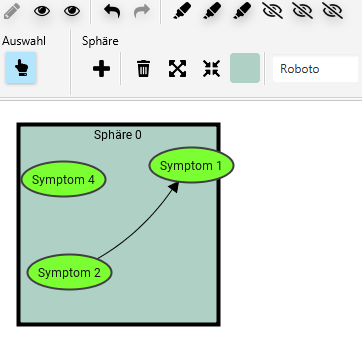
\includegraphics[width=0.4\columnwidth, keepaspectratio]{pick.png} 
		}
		\subfigure[Alternative 2]{
			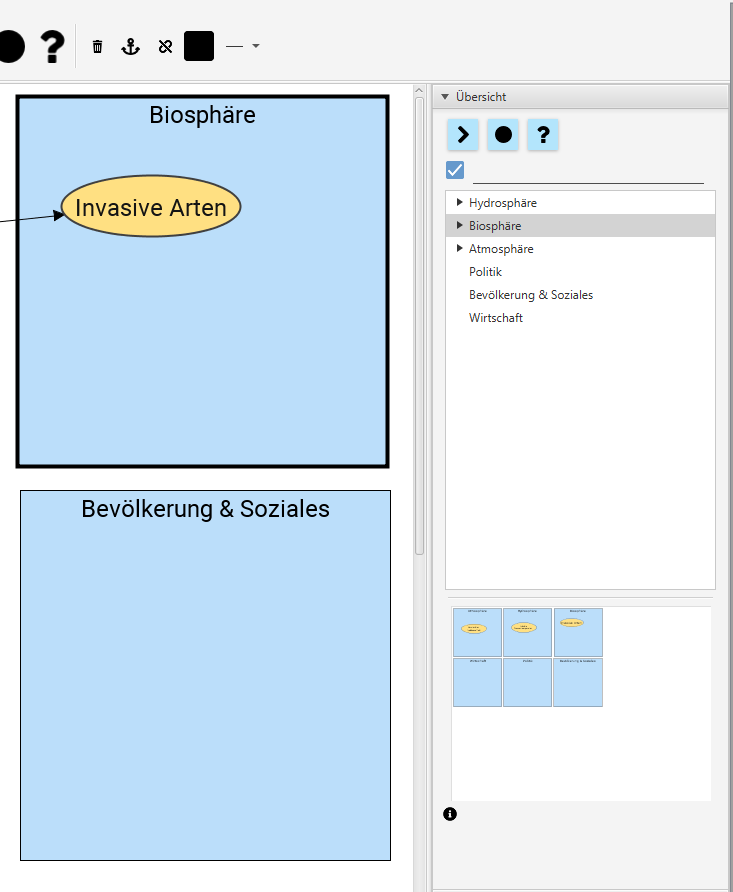
\includegraphics[width=0.4\columnwidth, keepaspectratio]{pick2.png} 
		}
		
	\end{figure}	
	%%%%%%%%%%%%%%%%%%%%%%%%%%%%%%%%%%%%%%%%%%%%%%%%%%%%%%%%%%%%%%%%%%%%%%% 	
	
	\newpage
	\subsubsection{Mehrerer Elemente}
	\condition
	Es muss ein Syndrom mit mindestens zwei Elemente (Sphären/ Symptome/ Relationen), welches ausgewählt werden soll, existieren. 
	\action
	\begin{enumerate}
		\item In der Menüleiste den Button \textit{Auswahl} durch einen Links-Klick aktivieren. 
		\item Auf der Tastatur den die Taste \texttt{Shift} gedrückt halten. 
		\item Den Cursor auf das Element bewegen, welches zur Auswahl hinzugefügt werden soll, und die linke Maustaste klicken. 
		\item Die \texttt{Shift} Taste solange gedrückt halten, wie Elemente der Auswahl hinzugefügt werden sollen.
		\item Die \texttt{Shift} Taste loslassen.
	\end{enumerate}
	\hint
	\begin{itemize}
		\item Verschiedene Arten (Sphären/ Symptome/ Relationen) von Graphelementen können in einer Aktion der Auswahl hinzugefügt werden. \\
	\end{itemize}

	\subsubsection{Auswahl löschen}
	\red{TODO}
	
		\newpage
%%%%%%%%%%%%%%%%%%%%%%%%%%%%%%%%%%%%%%%%%%%%%%%%%%%%%%%%%%%%%%%%%%%%%%%%%%%%%%%%%%%%%%%%%%%%%%%%%%%%%%%%
		\subsection{Nutzung der Übersichtsleiste} \label{overwiew}
		Die Übersichtsleiste befindet sich am rechten Rand der Anwendung. Über diese Leiste kann ein Element des Syndroms sowohl ausgewählt als auch dessen Eigenschaften verändert werden. Des weiteren kann es als zusätzliche Hilfe herangezogen werden, um die Struktur des Syndroms zu untersuchen. \\
		So kann über diese Leiste (zusätzlich zur visuellen Darstellung des Syndroms) ermittelt werden, welche Sphäre, welche Symptome enthält und welche Symptome durch Relationen verbunden sind. In diesem Fenster ist auch ein Filter integriert. Die Filterfunktion kann durch entsprechende Eingaben die Beschriftung von Symptomen und die Relationstypen der Relationen filtern.
		
		\begin{figure}[ht!]
			\centering
			\subfigure[Übersichtsleiste]{
				
\includegraphics[width=0.4\columnwidth, keepaspectratio]{placeholder.png} 
			}
			
		\end{figure}


%%%%%%%%%%%%%%%%%%%%%%%%%%%%%%%%%%%%%%%%%%%%%%%%%%%%%%%%%%%%%%%%%%%%%%%%%%%%%%%%%%%
\subsubsection{Navigation}		
	\condition
	Es muss ein Syndrom mit mindestens einer Sphäre im Programm geöffnet sein, damit die Übersichtsleiste nicht leer ist. 
	\action
	\begin{enumerate}
		\item In der Übersichtsleiste die Sphäre, zu der man die ihre zugeordneten Symptome angezeigt bekommen möchte, ausklappen. 
		\item Zum Schließen der Liste der Symptome die Sphäre einklappen. 
		\item Alternativ ein Symptom ausklappen, um die Liste der Relationen, die von ihm ausgehen, angezeigt zu bekommen. 
	\end{enumerate}
	\hint
	\begin{itemize}
		\item Element in der Übersichtsleiste können entweder durch einen Doppelklick der linken Maustaste oder durch einen Links-Klick auf das danebenstehende Pfeilsymbol ausgeklappt/ eingeklappt werden. 
		\item Ist in der Übersichtsleiste kein Pfeil vor einem Eintrag eingeblendet, so lässt sich dieses nicht ein-/ausklappen.
		\item Die Elemente eines Syndroms werden durch ihre Bezeichnung in der Übersichtleiste repräsentiert. Die Relationen werden durch ihr ausgehendes/ eingebendes Symptom identifiziert.\\
	\end{itemize}
		 
%%%%%%%%%%%%%%%%%%%%%%%%%%%%%%%%%%%%%%%%%%%%%%%%%%%%%%%%%%%%%%%%%%%%%%%%%%%%%%%%%%%
\subsubsection{Auswahl von Graphelementen}		
	\condition
	Es muss ein Syndrom mit mindestens einer Sphären im Programm geöffnet sein, damit die Übersichtsleiste nicht leer ist. 
	\action
	\begin{enumerate}
		\item In der Übersichtsleiste auf die eben beschriebene Weise bis zu der gewünschten Tiefe (nur Sphären, Symptome zu einer Sphäre, Relationen zu einem Symptom) navigieren. Dort das gewünschte Element wahlweise mit einem einfachen Links-Klick oder einem Doppelklick auswählen.
		\end{enumerate}
	\hint
	\begin{itemize}
		\item Das jeweils aktuell in der Übersichtsleiste ausgewählte Element wird auch in der (visuellen) Darstellung des Syndroms ausgewählt.\\
	\end{itemize}
		
%%%%%%%%%%%%%%%%%%%%%%%%%%%%%%%%%%%%%%%%%%%%%%%%%%%%%%%%%%%%%%%%%%%%%%%%%%%%%%%%%%%
\subsubsection{Filtern}
	\condition
	Es muss ein Syndrom mit mindestens einer Sphären im Programm geöffnet sein, damit die Übersichtsleiste nicht leer ist. 
	\actions
	\bbe{Filtern der Relationstypen:}
	\begin{enumerate}
		\item In der Übersichtsleiste einen Links-Klick in die Check-Box neben dem \textit{Nach der Pfeilspitze der Relation filtern}-Button ausführen, sodass dort ein Häkchen gesetzt ist.
		\item In der Übersichtsleiste einen Links-Klick auf den Button \textit{Nach der Pfeilspitze der Relation filtern} das Drop-Down-Menü dieses Buttons öffnen.
		\item In dem Drop-Down-Menü, den Relationstyp, der gefiltert werden soll, mit einem Links-Klick auswählen.
		\item Um wieder die Relationen aller Relationstypen einzublenden, erneut einen Links-Klick in die Check-Box neben dem \textit{Nach der Pfeilspitze der Relation filtern}-Button ausführen, sodass der Haken in dieser Box verschwindet.
	\end{enumerate}
	\bbe{Filtern der Symptome durch einen regulären Ausdruck:}
		\begin{enumerate}
		\item In der Übersichtsleiste einen Links-Klick in die Check-Box neben dem \textit{Nach regulären Ausdrücken filtern}-Feld ausführen, sodass dort ein ein Häkchen gesetzt ist.
		\item In der Übersichtsleiste einen Links-Klick in das Feld \textit{Nach regulären Ausdrücken filtern} ausführen.
		\item Über die Computertastatur einen Suchbegriff eingeben, nach dem der Titel von Symptomen gefiltert werden soll. 
		\item Um wieder alle Symptome einzublenden, erneut einen Links-Klick in die Check-Box neben dem \textit{Nach regulären Ausdrücken filtern}-Feld ausführen, sodass der Haken in dieser Box verschwindet.
		\end{enumerate}
	\hint
	\begin{itemize}
		\item Der ausgewählte Relationstyp wird weiterhin im Graphen angezeigt. Die Relationen der anderen beiden Relationstypen werden ausgeblendet. Diese Ausblendung gilt sowohl für die visuelle Darstellung des Syndroms im Hauptfenster als auch für die Liste der Relationen in der Übersichtsleiste.
		\item Die Symptome, deren Titel den Suchbegriff enthalten, werden weiterhin im Graphen angezeigt. Die übrigen Symptome werden ausgeblendet. Diese Ausblendung gilt sowohl für die visuelle Darstellung des Syndroms im Hauptfenster als auch für die Liste der Symptome in der Übersichtsleiste.
		\item In das Feld \textit{Nach regulären Ausdrücken filtern} können auch alle Form von regulären Ausdrücken eingegeben werden, z.B. \textbackslash d um nach Zahlen zu filtern)
		\item In beiden Filtervorgängen könne die ersten beiden Schritte auch in umgekehrter Reihenfolge durchgeführt werden.
		\item Das Ergebnis der Filterung schlägt sich sowohl in der Liste der Graphelemente in der Übersichtsleiste nieder als auch in der visuellen Darstellung des Syndroms.\\
	\end{itemize}		
		
%%%%%%%%%%%%%%%%%%%%%%%%%%%%%%%%%%%%%%%%%%%%%%%%%%%%%%%%%%%%
	\subsection{Editierung des Graphen - Allgemein}\label{edit}

		\red{\textbf{Hinweise}}
		\begin{itemize}
			\item In den folgenden Anleitungen wird immer davon ausgegangen, dass sich der Benutzer im \\
			Bearbeiter-/ Erstellermodus befindet und er somit die Berechtigung hat den Graphen zu editieren.
			\item Es wird vorausgesetzt, dass die Aktionen nicht durch die Vorlageregeln verhindert werden. D.h. das der Bearbeiter auf alle Elemente des Graphen freien Zugriff hat und alle Eigenschaften veränderbar sind.
			\item \bbe{Alle Aktionen die im folgenden beschrieben sind und sich auf die Editierung von Graphelementen beziehen sind auch auf eine Auswahl von mehreren Graphelementen ausführbar!}
		\end{itemize}
	
%%%%%%%%%%%%%%%%%%%%%%%%%%%%%%%%%%%%%%%%%%%%%%%%%%%%%%%%%%%%%%%%%%%%%%	
		\subsubsection{Undo/ Redo}
		Mit Undo/ Redo sind Aktionen auf dem Graphen wieder rückgängig zu machen oder rückgängig gemachte Aktionen erneut ausführbar. 
		\condition
		Es ist eine Aktions- Historie verfügbar. Beispiel: Es wurde ein Graph neu erstellt und eine Sphäre hinzugefügt. 	
		\action
		\begin{enumerate}
			\item Den Undo- Button durch einen Link-Klick auswählen. 
			\item Der Redo- Button sollte nun ebenfalls klickbar sein. Um die vorherige Aktion wieder auszuführen den Redo- Button klicken. 
		\end{enumerate}	
		\hint
		\begin{itemize}
			\item Die Aktions- Historie wird nach dem Wechsel in einen anderen Funktionsmodus oder nach dem Öffnen/ Importieren eines neuen Graphen gelöscht. \\ 
		\end{itemize}		
					
				\newpage
%%%%%%%%%%%%%%%%%%%%%%%%%%%%%%%%%%%%%%%%%%%%%%%%%%%%%%%%%%%%%%%%%%%%%%%%%%%%%%%%%%%%%%%
\subsubsection{Kontextmenü öffnen}
		\condition 	
		Ein Syndrom mit mindestens einer Sphäre und beliebig vielen weiteren Graphelementen ist im Programm geöffnet.
		\action
		\begin{enumerate}
				\item Das Graphelement, dessen Kontextmenü geöffnet werden soll, mit einem Rechts-Klick selektieren.
		\end{enumerate}
		\hint
		\begin{itemize}
				\item Es kann nur das Kontextmenü eines Graphelements zur jedem Zeitpunkt geöffnet werden.
				\item Die Kontextmenüs von Sphären, Symptomen und Relationen unterscheiden sich in ihrem Funktionsumfang.
				\item \bbe{Das Kontextmenü lässt sich an zwei verschieden Stellen öffen:} Zum einen im Hauptfenster, in dem der Graph visuell dargestellt wird, und zum anderen in der Übersichtsleiste. In beiden Fallen lässt es sich durch einen Rechts-Klick auf das entsprechende Element öffnen. \\
	 	\end{itemize}	 	
		
		
%%%%%%%%%%%%%%%%%%%%%%%%%%%%%%%%%%%%%%%%%%%%%%%%%%%%%%%%%%%%%%%%%%%%%%%%%%%%%%%%%%%%%%%%%%%%%%%%%%%%%%%%%%%%%
\subsection{Editierung der Sphären} \label{sphere}	
\subsubsection{Sphäre hinzufügen}	
		\condition 	
		Das Programm ist gestartet.
		\action
		\begin{enumerate}
			\item In der Menüleiste den Button \textit{Sphäre hinzufügen} durch einen Links-Klick aktivieren.
			\item Den Cursor auf die gewünschte Position bewegen, an der sich keine andere Sphäre befindet, und auf die linke Maustaste klicken.
		\end{enumerate}
		\hint
		\begin{itemize}
			\item Es ist nicht möglich eine Sphäre auf einer anderen Sphäre hinzuzufügen. Wird dies versucht, wird keine neue Sphäre hinzugefügt und es erscheint eine Fehlermeldung.
			\item Die Darstellung (Farbe, Kantenart, Typ) der Sphäre wird aus den ausgewählten Werten auf der Benutzeroberfläche ermittelt. \\
	\end{itemize}
	
	
%%%%%%%%%%%%%%%%%%%%%%%%%%%%%%%%%%%%%%%%%%%%%%%%%%%%%%%%%%%%%%%%%%%%%%%%%%%%%%%%%%%%%%%%%%%%%%%%%%%%%%%%%%%%%	
\subsubsection{Sphäre entfernen}
			\condition 	
		Ein Syndromansatz mit mindestens einer Sphäre ist im Programm geöffnet. 
		\actions  
		\aOne
		\begin{enumerate}
			\item Die Sphäre, die gelöscht werden soll mit einem Links-Klick auswählen.
			\item Die \textit{Entfernen}-Taste auf der Tastatur drücken.
		\end{enumerate}
	\newpage
		\hspace{-0.4cm}\aTwo
			\begin{enumerate}
			\item Die Sphäre, die gelöscht werden soll mit einem Links-Klick auswählen.
			\item In der Menüleiste einen Links-Klick auf den Button \textit{Sphäre löschen} ausführen.
		\end{enumerate}
		\aThree
		\begin{enumerate} 
			\item In diesem Kontextmenü der zu löschenden Sphäre die \textit{Entfernen}-Option mit einem Links-Klick auswählen.
		\end{enumerate}
		\hint
		\begin{itemize}
			\item Wird eine Sphäre gelöscht, so werden automatisch auch alle Symptome entfernt, die zu dieser Sphäre gehören. Damit werden dann auch alle Relationen gelöscht, die in einem dieser Symptome einmünden oder von einem dieser Symptome ausgehen.\\
		\end{itemize}
			
%%%%%%%%%%%%%%%%%%%%%%%%%%%%%%%%%%%%%%%%%%%%%%%%%%%%%%%%%%%%%%%%%%%%%%%%%%%%%%%%%%%%%%%%%%%%%%%%%%%%%%%%%%%%%	
\subsubsection{Sphäre verschieben}
		\condition 	
		Ein Syndrom mit mindestens einer Sphäre ist im Programm geöffnet. 
		\action  
		\begin{enumerate}
			\item Die Sphäre, die verschoben werden soll mit einem Rechts-Klick auswählen.
			\item Die (rechte) Taste gedrückt halten und den Cursor an eine Zielstelle bewegen, an der sich keine andere Sphäre befindet. Beim Bewegen des Cursors bewegt sich die Sphäre bereits mit. 
			\item Die rechte Maustaste loslassen.
		\end{enumerate}
		\hint
		\begin{itemize}
			\item Es ist nicht möglich, eine Sphäre zu verschieben, wenn sich an der Zielposition bereits eine andere Sphäre befindet. Wird dies versucht, wird die Sphäre nicht verschoben und es erscheint eine Fehlermeldung.\\
		\end{itemize}
			
%%%%%%%%%%%%%%%%%%%%%%%%%%%%%%%%%%%%%%%%%%%%%%%%%%%%%%%%%%%%%%%%%%%%%%%%%%%%%%%%%%%%%%%%%%%%%%%%%%%%%%%%%%%%%	
\subsubsection{Größe einer Sphäre verändern}
				\condition 	
		Ein Syndrom mit mindestens einer Sphäre ist im Programm geöffnet. 
		\actions  
		\aOne
		\begin{enumerate}
			\item Die Sphäre, deren Größe verändert werden soll, mit einem Links-Klick auswählen.
			\item So oft die \glqq\textit{+}\grqq- / \glqq\textit{-}\grqq-Taste der Tastatur drücken bis die Sphäre die gewünschte Größe hat. \\(Nicht die \glqq\textit{+}\grqq- / \glqq\textit{-}\grqq-Taste des Nummernblocks)
		\end{enumerate}
		\aTwo
			\begin{enumerate}
			\item Die Sphäre, deren Größe geändert werden soll, mit einem Links-Klick auswählen.
			\item In der Menüleiste so oft  Links-Klick auf den Button \textit{Sphäre vergrößern}/\textit{Sphäre verkleinern} ausführen bis die Sphäre die gewünschte Größe erreicht hat. 
		\end{enumerate}
		\hint
		\begin{itemize}
			\item Eine Sphäre kann nicht mehr verkleinert werden, wenn sie bereits ihre minimale Größe erreicht hat oder ein Symptom sich durch die Verkleinerung außerhalb der Sphäre befinden würde.
			\item Eine Sphäre kann nicht weiter vergrößert werden, wenn die Vergrößerung zu einer Überlappung von zwei Sphären führen würde.\\
		\end{itemize}
				
%%%%%%%%%%%%%%%%%%%%%%%%%%%%%%%%%%%%%%%%%%%%%%%%%%%%%%%%%%%%%%%%%%%%%%%%%%%%%%%%%%%%%%%%%%%%%%%%%%%%%%%%%%%%%	
\subsubsection{Farbe einer Sphäre ändern}
		\condition 	
		Ein Syndrom mit mindestens einer Sphäre ist im Programm geöffnet. 
		\actions  
		\aOne
		\begin{enumerate}
			\item In der Menüleiste mit der linken Maustaste auf den Button \textit{Hintergrundfarbe der Sphäre verändern} klicken und eine Farbe auswählen.
			\item Das Kontextmenü der Sphäre, deren Farbe geändert werden soll, öffnen und dort den Punkt \textit{Farbe} auswählen.
		\end{enumerate}
		\aTwo
		\begin{enumerate}
			\item Die Sphäre, deren Farbe geändert werden soll, mit einem Links-Klick auswählen.
			\item In der Menüleiste mit der linken Maustaste auf den Button \textit{Hintergrundfarbe der Sphäre verändern} klicken und eine Farbe auswählen.
		\end{enumerate}
		\hint
		\begin{itemize}
			\item Wenn die gewünschte Farbe nicht in dem sich öffnenden Fenster enthalten ist, lässt sich ein weiteres Farbwahl-Fenster durch einen Links-Klick auf \textit{Custom Color} öffnen. Die Bedienung des Color Pickers ist im Kapiel \nameref{colorpicker} beschrieben.\\
	\end{itemize}	
	
%%%%%%%%%%%%%%%%%%%%%%%%%%%%%%%%%%%%%%%%%%%%%%%%%%%%%%%%%%%%%%%%%%%%%%%%%%%%%%%%%%%%%%%%%%%%%%%%%%%%%%%%%%%%%%	
\subsubsection{Titel einer Sphäre ändern}
				\condition 	
		Ein Syndrom mit mindestens einer Sphäre ist im Programm geöffnet. 
		\action  
		\begin{enumerate}
			\item Das Kontextmenü der Sphäre, deren Titel geändert werden soll, öffnen und dort die \textit{Titel}-Option mit einem Links-Klick auswählen. 
			\item In dem sich öffnenden Fenster für die gewünschten Sprache(n) den neuen Titel in die dafür vorgesehenen Felder eingeben.
			\item Die Änderung des Titels mit einem Links-Klick auf die \textit{Speichern}-Schaltfläche abschließen.
		\end{enumerate}
		\hint
		\begin{itemize}
			\item Der Titel einer Sphäre darf kein Semikolon enthalten und nicht leer sein.
			\item Doppelte Bezeichnungen sind in einem Syndrom nicht erlaubt. Bei Eingabe eines doppelt vorkommenden Titels erscheint in dem Dialogfenster eine Fehlermeldung und der \textit{Speichern} -Button ist nicht mehr auswählbar bis der Titel entsprechend geändert wurde. \\
		\end{itemize}	
			
%%%%%%%%%%%%%%%%%%%%%%%%%%%%%%%%%%%%%%%%%%%%%%%%%%%%%%%%%%%%%%%%%%%%%%%%%%%%%%%%%%%%%%%%%%%%%%%%%%%%%%%%%%%%%%%%%%%%%%%%%%%%%5			
\subsubsection{Schriftart/-größe der Beschriftung einer Sphäre ändern}
		\condition 	
		Ein Syndrom mit mindestens einer Sphäre ist im Programm geöffnet. 
		\actions  
		\aOne
		\begin{enumerate}
			\item Die Sphäre, für die die Schriftart/-größe geändert werden soll, mit einem Links-Klick auswählen.
			\item In der Menüleiste einen Links-Klick auf das Feld klicken, in dem die Schriftart/-größe von Sphären angezeigt wird.
			\item In dem Drop-Down-Menü die Schriftart/-größe auswählen, welche die Beschriftung der Sphäre haben soll.
		\end{enumerate}
		\aTwo
		\begin{enumerate}
			\item In der Menüleiste einen Links-Klick auf das Feld klicken, in dem die aktuelle Schriftart/-größe der Sphäre angezeigt wird.
			\item In dem Drop-Down-Menü die Schriftart/-größe auswählen, indem die Schriftart/-größe von Sphären angezeigt wird.
			\item Das Kontextmenü der Sphäre öffnen, deren Schriftart/-größe geändert werden soll und dort die Option \textit{Schriftart}/\textit{Schriftgröße} auswählen. \\
		\end{enumerate}
			
%%%%%%%%%%%%%%%%%%%%%%%%%%%%%%%%%%%%%%%%%%%%%%%%%%%%%%%%%%%%%%%%%%%%%%%%%%%%%%%%%%%%%%%%%%%%%%%%%%%%%%%%%%%%%	
		\subsubsection{Sphären layouten}
		\condition 	
		Ein Syndrom mit mindestens einer Sphäre ist im Programm geöffnet. 
		\action  
		\begin{enumerate}
			\item In der Menüleiste im Bereich Sphären auf den \textit{Automatische Anordnung}-Button mit Links-Klick klicken.
		\end{enumerate}
		\hint
		\begin{itemize}
			\item Wenn die Position von einer Sphäre aufgrund der Vorlageregeln gesperrt ist, dann steht dem Bearbeiter diese Funktion nicht mehr zur Verfügung. \\
		\end{itemize}		
			
				
%%%%%%%%%%%%%%%%%%%%%%%%%%%%%%%%%%%%%%%%%%%%%%%%%%%%%%%%%%%%%%%%%%%%%%%%%%%%%%%%%%%%%%%%%%%%%%%%%%%%%%%%%%%%%	
\subsection{Editierung der Symptome} \label{symptom}
		\subsubsection{Symptom hinzufügen}
		\condition 	
		Ein Syndrom mit mindestens einer Sphäre ist im Programm geöffnet. 
		\action
		\begin{enumerate}
			\item In der Menüleiste den Button \textit{Symptom hinzufügen} durch einen Links-Klick aktivieren.
			\item Den Cursor auf die gewünschte Position innerhalb einer Sphäre bewegen, an der sich kein(e) andere(s) Symptom / Relation befindet, und auf die linke Maustaste klicken.
		\end{enumerate}
		\hint
		\begin{itemize}
			\item Es ist nicht möglich, ein Symptom auf einen anderem Symptom hinzuzufügen. Wird dies versucht, wird kein neues Symptom hinzugefügt und es erscheint eine Fehlermeldung.
			\item Es ist nicht möglich, ein Symptom außerhalb einer Sphäre hinzuzufügen. Wird dies versucht, wird kein neues Symptom hinzugefügt und es erscheint eine Fehlermeldung.
			\item Es ist nicht möglich ein Symptom auf einer Relation hinzuzufügen. Wird dies versucht, wird kein neues Symptom hinzugefügt und es erscheint eine Fehlermeldung.
			\item Die Darstellung (Farbe, Kantenart, Typ) des Symptoms wird aus den ausgewählten Werten auf der Benutzeroberfläche ermittelt. \\
		\end{itemize}

%%%%%%%%%%%%%%%%%%%%%%%%%%%%%%%%%%%%%%%%%%%%%%%%%%%%%%%%%%%%%%%%%%%%%%%%%%%%%%%%%%%%%%%%%%%%%%%%%%%%%%%%%%%%%	
\subsubsection{Symptom entfernen}
		\condition 	
		Ein Syndrom mit mindestens einer Sphäre, die ein oder mehr Symptome enthält, ist im Programm geöffnet. 
		\actions
		\aOne
		\begin{enumerate}
			\item Das Symptom, welches gelöscht werden soll mit einem Links-Klick auswählen. 
			\item Die \textit{Entfernen}-Taste der Tastatur drücken.
		\end{enumerate}
		\aTwo
		\begin{enumerate}
			\item Das Symptom, welches gelöscht werden soll mit einem Links-Klick auswählen. 
			\item In der Menüleiste den \textit{Symptom löschen}-Button durch einen Links-Klick auslösen.
		\end{enumerate}
		\aThree
			\begin{enumerate} 
				\item In dem Kontextmenü des zu löschenden Symptoms die \textit{Entfernen}-Option mit einem Links-Klick auswählen.
			\end{enumerate}
		\hint
		\begin{itemize}
			\item Beim Löschen eines Symptoms werden auch alle von dem Symptom ausgehenden Kanten gelöscht. \\
		\end{itemize}
		
%%%%%%%%%%%%%%%%%%%%%%%%%%%%%%%%%%%%%%%%%%%%%%%%%%%%%%%%%%%%%%%%%%%%%%%%%%%%%%%%%%%%%%%%%%%%%%%%%%%%%%%%%%%%%	
\subsubsection{Symptom verschieben}
		\condition 	
		Ein Syndrom mit mindestens einer Sphäre, die ein oder mehr Symptome enthält, ist im Programm geöffnet. 
		\action
		\begin{enumerate}
			\item Das Symptom, welches verschoben werden soll mit einem Rechts-Klick auswählen. 
			\item Die rechte Maustaste gedrückt halten und den Cursor an die Stelle bewegen, an der es platziert werden soll.
			\item Die rechte Maustaste loslassen. 
		\end{enumerate}
		\hint
		\begin{itemize}
			\item Es ist nicht möglich, ein Symptom auf die Position eines anderen Symptoms zu verschieben. Wird dies versucht, wird das Symptom an seiner ursprünglichen Stelle platziert und es erscheint eine Fehlermeldung.
			\item Es ist nicht möglich, ein Symptom außerhalb einer Sphäre zu platzieren. Wird dies versucht, wird das Symptom an seiner ursprünglichen Stelle platziert und es erscheint eine Fehlermeldung.
		\end{itemize}
		
%%%%%%%%%%%%%%%%%%%%%%%%%%%%%%%%%%%%%%%%%%%%%%%%%%%%%%%%%%%%%%%%%%%%%%%%%%%%%%%%%%%%%%%%%%%%%%%%%%%%%%%%%%%%%	
\subsubsection{Größe eines Symptoms verändern}
					\condition 	
		Ein Syndrom mit mindestens einer Sphäre, die ein oder mehr Symptome enthält, ist im Programm geöffnet. 
		\actions
		\aOne
		\begin{enumerate}
			\item Das Symptom, dessen Größe verändert werden soll, mit einem Links-Klick auswählen. 
			\item Die \glqq\textit{+}\grqq- / \glqq\textit{-}\grqq-Taste der Tastatur so oft drücken bis das Symptom die gewünschte Größe erreicht hat. (Nicht die  \glqq\textit{+}\grqq- / \glqq\textit{-}\grqq-Taste des Nummernblocks)
		\end{enumerate}
		\aTwo
		\begin{enumerate}
			\item Das Symptom, dessen Größe verändert werden soll, mit einem Links-Klick auswählen. 
			\item  In der Menüleiste den \textit{Symptom vergrößern}- / \textit{Symptom verkleinern}-Button klicken so oft drücken bis das Symptom die gewünschte Größe erreicht hat.
		\end{enumerate}
		\hint
		\begin{itemize}
			\item Es ist nicht möglich, ein Symptom zu verkleinern, wenn es bereits seine minimale Größe hat oder die Beschriftung die aktuelle Größe mindestens erfordert. \\
		\end{itemize}
			
%%%%%%%%%%%%%%%%%%%%%%%%%%%%%%%%%%%%%%%%%%%%%%%%%%%%%%%%%%%%%%%%%%%%%%%%%%%%%%%%%%%%%%%%%%%%%%%%%%%%%%%%%%%%%	
\subsubsection{Füllfarbe/ Randfarbe eines Symptoms verändern}
		\condition 	
		Ein Syndrom mit mindestens einer Sphäre, die ein oder mehr Symptome enthält, ist im Programm geöffnet. 
		\actions
		\aOne
		\begin{enumerate}
			\item In der Menüleiste mit der linken Maustaste auf den Button \textit{Hintergrundfarbe des Symptoms verändern}/ \textit{Randfarbe des Symptoms verändern} klicken und eine Farbe auswählen.
			\item Mit einem Rechts-Klick auf das Symptom, dessen Farbe geändert werden soll, dessen Kontextmenü öffnen.
			\item In dem Kontextmenü den Punkt \textit{Füllfarbe}/ \textit{Randfarbe} auswählen.
		\end{enumerate}		
		\aTwo
		\begin{enumerate}
			\item Das Symptom, dessen Farbe geändert werden soll, mit einem Links-Klick auswählen.
			\item In der Menüleiste mit der linken Maustaste auf den Button \textit{Hintergrundfarbe des Symptoms verändern}/ \textit{Randfarbe des Symptoms verändern} klicken.
			\item In dem sich öffnenden Fenster die gewünschte Farbe mit einem Links-Klick auswählen.
		\end{enumerate}
		
		\hint
		\begin{itemize}
			\item Die Bedienung des Farbwahl-Fensters ist im Kapitel \nameref{colorpicker} beschrieben. \\
		\end{itemize}		
		
%%%%%%%%%%%%%%%%%%%%%%%%%%%%%%%%%%%%%%%%%%%%%%%%%%%%%%%%%%%%%%%%%%%%%%%%%%%%%%%%%%%%%%%%%%%%%%%%%%%%%%%%%%%%%		
\subsubsection{Titel eines Symptoms ändern}
		\condition 	
		Ein Syndrom mit mindestens einer Sphäre, die ein oder mehr Symptome enthält, ist im Programm geöffnet. 
		\action 
		\begin{enumerate}
			\item Das Symptom, dessen Titel geändert werden soll mit einem Rechts-Klick anklicken, sodass sich dessen Kontextmenü öffnet.
			\item Im Kontextmenü ganz oben \textit{Titel} mit einem Links-Klick auswählen. 
			\item In dem sich öffnenden Fenster für die gewünschten Sprache(n) den neuen Titel in die dafür vorgesehenen Felder eingeben.
			\item Die Änderung des Titels mit einem Links-Klick auf die \textit{Speichern}-Schaltfläche abschließen.
		\end{enumerate}
		\hint
		\begin{itemize}
			\item Der Titel eines Symptoms darf kein Semikolon enthalten und nicht leer sein. 
			\item Doppelte Bezeichnungen sind in einem Syndrom nicht erlaubt. Bei Eingabe eines doppelt vorkommenden Titels erscheint in einem Dialogfenster eine Fehlermeldung und der \textit{Speichern} -Button ist nicht mehr auswählbar bis die Eingabe entsprechend geändert wurde. \\
		\end{itemize}
			
%%%%%%%%%%%%%%%%%%%%%%%%%%%%%%%%%%%%%%%%%%%%%%%%%%%%%%%%%%%%%%%%%%%%%%%%%%%%%%%%%%%%%%%%%%%%%%%%%%%%%%%%%%%%%	
\subsubsection{Schriftart/-größe der Beschriftung eines Symptoms ändern}
		\condition 	
		Ein Syndrom mit mindestens einer Sphäre, die ein oder mehr Symptome enthält, ist im Programm geöffnet. 
		\actions  
		\aOne
		\begin{enumerate}
			\item Das Symptom, für das die Schriftart/-größe geändert werden soll, mit einem Links-Klick auswählen.
			\item In der Menüleiste einen Links-Klick auf das Feld klicken, in dem die Schirftart/ -größe von Symptomen angezeigt wird. 
			\item In dem Drop-Down-Menü die Schrifart/-größe auswählen, die die Beschriftung des Symptoms haben soll.
		\end{enumerate}
		\aTwo
			\begin{enumerate}
			\item In der Menüleiste einen Links-Klick auf das Feld klicken, in dem die Schirftart/ -größe von Symptomen angezeigt wird. 
			\item In dem Drop-Down-Menü die Schrifart/-größe auswählen, die die Beschriftung des Symptoms haben soll.
			\item Mit einem Rechts-Klick auf das Symptom klicken, dessen Schriftart/-größe geändert werden soll.
			\item In dem sich öffnenden Kontextmenü die Option \textit{Schriftart}/\textit{Schriftgröße} auswählen.
		\end{enumerate}
			
%%%%%%%%%%%%%%%%%%%%%%%%%%%%%%%%%%%%%%%%%%%%%%%%%%%%%%%%%%%%%%%%%%%%%%%%%%%%%%%%%%%%%%%%%%%%%%%%%%%%%%%%%%%%%	
\subsubsection{Form eines Symptoms verändern}
		\condition 	
		Ein Syndrom mit mindestens einer Sphäre, die ein oder mehr Symptome enthält, ist im Programm geöffnet. 
		\action
		\begin{enumerate}
			\item Das Symptom, dessen Form geändert werden soll mit einem Rechts-Klick auswählen. 
			\item In der Menüleiste den Button \textit{Form des Symptoms verändern} anklicken.
			\item In dem sich öffnenden Drop-Down-Menü die Form auswählen, die das Symptom haben soll. \\
		\end{enumerate}
	
%%%%%%%%%%%%%%%%%%%%%%%%%%%%%%%%%%%%%%%%%%%%%%%%%%%%%%%%%%%%%%%%%%%%%%%%%%%%%%%%%%%%%%%%%%%%%%%%%%%%%%%%%%%%%		
		\subsubsection{Symptome layouten}
		\condition 	
		Ein Syndrom mit mindestens zwei Symptome und durch eine Relation verbunden sind, ist im Programm geöffnet. 
		\action 
		\begin{enumerate}
			\item In der Menüleiste im Bereich Symptom den \textit{Automatische Anordnung} Button mit Links-Klick klicken.
		\end{enumerate}
		\hint
		\begin{itemize}
			\item Wurde bei einem der Symptome die Position durch die Vorlageregeln gelockt, ist der \textit{Automatische Anordnung} Button nicht mehr auswählbar.
			\item Es gibt nicht nur ein mögliches Layout für die gleiche Menge an Symptomen. Es können verschiedene Layouts berechnet werden. Bei erneuten Klick auf den \textit{Automatische Anordnung} Button wird sich deswegen das Layout/ die Anordnung der Symptome verändern. \\
		\end{itemize}	
			
%%%%%%%%%%%%%%%%%%%%%%%%%%%%%%%%%%%%%%%%%%%%%%%%%%%%%%%%%%%%%%%%%%%%%%%%%%%%%%%%%%%%%%%%%%%%%%%%%%%%%%%%%%%%%	
\subsection{Editierung der Relationen} \label{relations}
		\subsubsection{Relation hinzufügen}
		\condition
		Um eine Relation hinzufügen zu können, müssen mindestens 2 Symptome im Syndrom existieren. 
		\action
		\begin{enumerate}
			\item Auf ein Symptom klicken und die Maustaste gedrückt halten.
			\item Die Maus zu einem zweiten Symptom bewegen. 
			\item Die Maustaste auf einem anderem Symptom loslassen. 
		\end{enumerate}
		\hint
		\begin{itemize}
			\item Die Darstellung (Farbe, Kantenart, Typ) der Relation wird aus den ausgewählten Werten auf der Benutzeroberfläche ermittelt. 
			\item Es können nur Relationen zwischen zwei Symptomen hinzugefügt werden. 
			\item Ein Symptom kann keine Relation auf sich selber haben.
			\item Die Ankerpunkte der Relationen (von dem ausgehenden/ eingehenden Symptom) werden automatisch gesetzt und können manuell durch den Benutzer im Nachhinein verändert werden. 
			\item Die Pfeile von Relationen des gleichen Typs werden dabei in einem bestimmten Bereich zusammengefasst dargestellt. 
			\item Pfeilspitzen verschiedenen Types sollen sich nicht überlappen.
		\end{itemize}
		
		\begin{figure}[ht!]
			\centering
			\subfigure[Relationen]{
				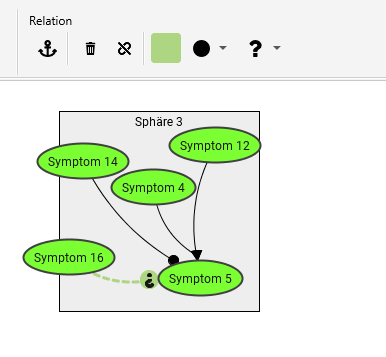
\includegraphics[width=0.4\columnwidth, keepaspectratio]{edge.png} 
			}			
		\end{figure}
		
%%%%%%%%%%%%%%%%%%%%%%%%%%%%%%%%%%%%%%%%%%%%%%%%%%%%%%%%%%%%%%%%%%%%%%%%%%%%%%%%%%%%%%%%%%%%%%%%%%%%%%%%%%%%%
		\subsubsection{Relation entfernen}
		\condition
		Es muss mindestens eine Relation in dem Syndrom existieren. 
		\actions
		\aOne
		\begin{enumerate}
			\item Die Relation, die gelöscht werden soll mit einem Links-Klick auswählen.
			\item Die \textit{Entfernen}-Taste auf der Tastatur drücken.
		\end{enumerate}
		\aTwo
		\begin{enumerate}
			\item Die Relation, welche gelöscht werden soll mit einem Links-Klick auswählen.
			\item In der Menüleiste einen Links-Klick auf den Button \textit{Relation entfernen} ausführen.
		\end{enumerate}
		\aThree
		\begin{enumerate}
			\item Mit einem Rechts-Klick auf die Relation, welche gelöscht werden soll, das Kontextmenü öffnen. 
			\item In diesem Kontextmenü die \textit{Entfernen}-Option mit einem Links-Klick auswählen. \\
		\end{enumerate}
		
%%%%%%%%%%%%%%%%%%%%%%%%%%%%%%%%%%%%%%%%%%%%%%%%%%%%%%%%%%%%%%%%%%%%%%%%%%%%%%%%%%%%%%%%%%%%%%%%%%%%%%%%%%%%%
\subsubsection{Ankerpunkte ein-/ ausblenden}
		Ankerpunkte bezeichnen die Postion, wo die Relation in einem Symptom mündet/ von ihm ausgeht. Bei der Erstellung einer Relation werden diese automatisch gesetzt und sind veränderbar. Das bedeutet, dass wenn ein Symptom bewegt wird, sich die Postion der Mündung/Ausgang der Relation in/aus das Symptom entsprechend anpasst und bewegt. Um das zu verhindert, können die Ankerpunkte manuell gesetzt werden. Diese sind dann fest, d.h. auch beim Bewegen eines Symptoms bleibt die Position der Mündung/ des Ausgangs bestehen.
		\condition
		Es muss mindestens eine Relation im Syndromansatz existieren und mindestens ein Ankerpunkt gesetzt sein. 
		\action
		\begin{enumerate}
			\item In der Menüleiste den Button \textit{Ankerpunkte ein-/ausblenden} durch einen Links- Klick aktivieren.
			\item Zum Ausblenden den Button durch einen Links- Klick deaktivieren. 
		\end{enumerate}
		\hint
		\begin{itemize}
			\item Die Ankerpunkte werden beim Einblenden rot eingefärbt. 
		\end{itemize}
		\begin{figure}[ht!]
			\centering
			\subfigure[Ankerpunkte]{
				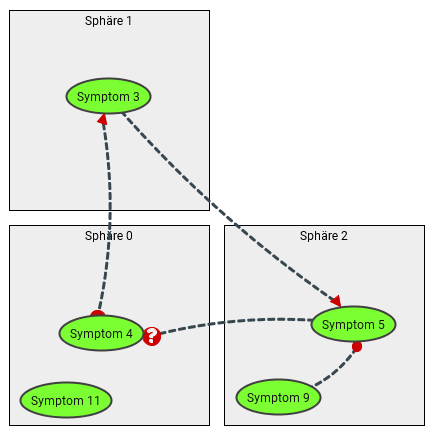
\includegraphics[width=0.4\columnwidth, keepaspectratio]{anchor.png} 
			}			
		\end{figure}
		
		\newpage
%%%%%%%%%%%%%%%%%%%%%%%%%%%%%%%%%%%%%%%%%%%%%%%%%%%%%%%%%%%%%%%%%%%%%%%%%%%%%%%%%%%%%%%%%%%%%%%%%%%%%%%%%%%%%	
\subsubsection{Ankerpunkte hinzufügen}
		\condition
		Es muss mindestens eine Relation im Syndromansatz existieren.
		\action
		\begin{enumerate}
			\item Die Kante durch einen Rechts- Klick auswählen und gedrückt halten.
			\item Befindet sich die Position der Maus beim Klick näher am Symptom, in welches die Relation mündet, wird der Ankerpunkt der Mündung der Relation gesetzt. Befindet sich die Position der Maus beim Klick näher am Symptom, von dem die Kante ausgeht, wird der Ankerpunkt für den Ausgang der Kante gesetzt. 
			\item Die Kante in die gewünschte Richtung bewegen. Die Mündung/ der Ausgang der Kante wandert entsprechend mit. 
			\item Wenn die gewünschte Position erreicht ist, die gedrückte Maustaste loslassen. 
		\end{enumerate}
		\begin{figure}[ht!]
			\centering
			\subfigure[Alternative 1]{
				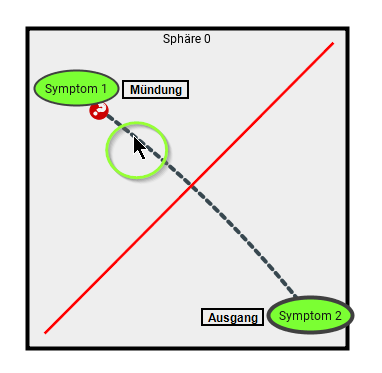
\includegraphics[width=0.3\columnwidth, keepaspectratio]{add_anchor.png} 
			}			
		\end{figure}
		\hint
		\begin{itemize}
			\item Beim Beispiel in der Abbildung wird aufgrund der Mausposition der Ankerpunkt bei der Mündung der Relation gesetzt. \\
		\end{itemize}
		
%%%%%%%%%%%%%%%%%%%%%%%%%%%%%%%%%%%%%%%%%%%%%%%%%%%%%%%%%%%%%%%%%%%%%%%%%%%%%%%%%%%%%%%%%%%%%%%%%%%%%%%%%%%%%
\subsubsection{Ankerpunkte entfernen}
		\condition
		Es muss mindestens eine Relation im Syndromansatz existieren.
		\action
		\begin{enumerate}
			\item Die gewünschte Relation durch einen Link- Klick auswählen. 
			\item In der Menüleiste einen Links-Klick auf den Button \textit{Ankerpunkt entfernen} ausführen.
		\end{enumerate}
		\hint
		\begin{itemize}
			\item Beim Entfernen der Ankerpunkte werden immer (wenn gesetzt) beide Ankerpunkte entfernt.\\
		\end{itemize}
		
%%%%%%%%%%%%%%%%%%%%%%%%%%%%%%%%%%%%%%%%%%%%%%%%%%%%%%%%%%%%%%%%%%%%%%%%%%%%%%%%%%%%%%%%%%%%%%%%%%%%%%%%%%%%%
\subsubsection{Farbe einer Relation verändern}
		\condition
		Es muss mindestens eine Relation im Syndromansatz existieren.
		\actions
		\aOne
		\begin{enumerate}
			\item In der Menüleiste mit der linken Maustaste auf den Button \textit{Farbe der Relation verändern} klicken.
			\item Mit einem Rechts-Klick auf die Relation, deren Farbe geändert werden soll, das Kontextmenü öffnen.
			\item Im Kontextmenü den Punkt \textit{Relationsfarbe} auswählen.
		\end{enumerate}
		\aTwo
		\begin{enumerate}
			\item Die Relation, deren Farbe geändert werden soll, mit einem Links-Klick auswählen.
			\item In der Menüleiste mit der linken Maustaste einen Links-Klick auf den Button \textit{Farbe der Relation verändern} ausführen.
			\item In dem sich öffnenden Fenster die gewünschte Farbe mit einem auswählen. \\
		\end{enumerate}	
		
%%%%%%%%%%%%%%%%%%%%%%%%%%%%%%%%%%%%%%%%%%%%%%%%%%%%%%%%%%%%%%%%%%%%%%%%%%%%%%%%%%%%%%%%%%%%%%%%%%%%%%%%%%%%%
\subsubsection{Type einer Relation verändern}
		\condition
		Es muss mindestens eine Relation im Syndromansatz existieren.
		\actions
		\aOne
		\begin{enumerate}
			\item In der Menüleiste mit der linken Maustaste auf den Button \textit{Typ der Relation verändern} klicken.
			\item Aus dem Drop-Down-Menü den gewünschten Typ per Links- Klick auswählen.
			\item Mit einem Rechts-Klick auf die Relation, deren Typ geändert werden soll, das Kontextmenü öffnen.
			\item Im Kontextmenü den Punkt \textit{Typ} auswählen.
		\end{enumerate}
		\aTwo
		\begin{enumerate}
			\item Die Relation, deren Typ geändert werden soll, mit einem Links-Klick auswählen.
			\item In der Menüleiste mit der linken Maustaste einen Links-Klick auf den Button \textit{Typ der Relation verändern} ausführen.
			\item Aus dem Drop-Down einen Typ per Links- Klick auswählen. 
		\end{enumerate}	
		\hint
		\begin{itemize}
			\item Die normale Pfeilspitze stellt die verstärkende Beziehung von Relationen im Syndromansatz dar.
			\item Die kreisförmige Pfeilspitze stellt die abschwächend Beziehung von Relationen im Syndromansatz dar.
			\item Die Pfeilspitze mit dem Fragezeichen stellt die neutrale Beziehung von Relationen im Syndromansatz dar.
		\end{itemize}
		
%%%%%%%%%%%%%%%%%%%%%%%%%%%%%%%%%%%%%%%%%%%%%%%%%%%%%%%%%%%%%%%%%%%%%%%%%%%%%%%%%%%%%%%%%%%%%%%%%%%%%%%%%%%%%
		\subsubsection{Graphelemente hervorheben}
		\condition 	
		Ein Syndrom mit mindestens einer Sphäre, die ein oder mehr Symptome und eine oder mehr Relationen enthält, ist im Programm geöffnet. 
		\actions
		Alternative 1:
		\begin{enumerate}
			\item Das Symptom / die Relation, das / die hervorgehoben werden soll, mit einem Links-Klick auswählen. 
			\item In der Menüleiste den Button \textit{Elemente hervorheben} klicken.
		\end{enumerate}
				Alternative 2:
		\begin{enumerate}
			\item Im Kontextmenü des Graphelements, das hervorgehoben werden soll, die Option \textit{Hervorhebung} mit einem Links-Klck auswählen.
		\end{enumerate}
		\hint
		\begin{itemize}
					\item Es können lediglich Symptome und Relationen und somit keine Sphären hervorgehoben werden
					\item Wird die Aktion auf einem Graphelement ausgeführt, das aktuell bereits hervorgehoben ist, passiert nichts.
					\item Um die Hervorhebung zu aktivieren / sichtbar zu machen den Button \textit{Hervorgehobene Elemente aktivieren} in der Menüleiste anklicken. Durch einen erneuten Klick auf diesen Button wird die Hervorhebung wieder deaktiviert. Dabei kann dieser \textit{Hervorgehobene Elemente aktivieren}-Button zu einem beliebigen Zeitpunkt im oben beschriebenen Ablauf geklickt werden.
					\item Es können mehrere Symptome und Relationen ausgewählt werden, die anschließend durch Klicken des \textit{Elemente hervorheben}-Button hervorgehoben werden, indem die \textit{Shift}-Taste gedrückt gehalten wird und die gewünschten Elemente jeweils mit einem Links-Klick ausgewählt werden.
		\end{itemize}
		
			\newpage
			
			subsection{Hervorheben und Ausblenden (symptome und Relationen)}
			
		%%%%%%%%%%%%%%%%%%%%%%%%%%%%%%%%%%%%%%%%%%%%%%%%%%%%%%%%%%%%%%%%%%%%%%%%%%%%%%%%%%%%%%%%%%%%%%%%%%%%%%%%%%%%%
		\subsubsection{Graphelemente zur Hervorhebung hinzufügen}
				\condition 	
		Ein Syndrom mit mindestens einer Sphäre, die ein oder mehr Symptome und eine oder mehr Relationen enthält, ist im Programm geöffnet. Es ist mindestens eines dieser Elemente hervorgehoben und eines noch nicht hervorgehoben.
		\actions
		Das Graphelement, das neben den bereits hervorgehobenen Elementen ebenfalls hervorgehoben werden soll, wie im vorangehenden Kapitel beschrieben hervorheben.
		\hint
		\begin{itemize}
					\item Die bereits hervorgehoben Elemente bleiben hervorgehoben.
		\end{itemize}
		
			\newpage
		%%%%%%%%%%%%%%%%%%%%%%%%%%%%%%%%%%%%%%%%%%%%%%%%%%%%%%%%%%%%%%%%%%%%%%%%%%%%%%%%%%%%%%%%%%%%%%%%%%%%%%%%%%%%%
		\subsubsection{Graphelemente aus der Hervorhebung entfernen}
			\condition 	
		Ein Syndrom mit mindestens einer Sphäre, die ein oder mehr Symptome und eine oder mehr Relationen enthält, ist im Programm geöffnet. Es ist mindestens eines dieser Elemente hervorgehoben.
		\actions
		Alternative 1:
		\begin{enumerate}
			\item Das Symptom / die Relation, das / die aktuell hervorgehoben ist und deren Hervorhebung aufgehoben werden soll, mit einem Links-Klick auswählen. 
			\item In der Menüleiste den Button \textit{Hervorhebung von Elementen entfernen} klicken.
		\end{enumerate}
				Alternative 2:
		\begin{enumerate}
			\item Im Kontextmenü des Graphelements, das aktuell hervorgehoben ist und dessen Hervorhebung aufgehoben werden soll, die Option \textit{Hervorhebung} mit einem Links-Klck auswählen.
		\end{enumerate}
		\hint
		\begin{itemize}
				\item Wird die Aktion auf einem Graphelement ausgeführt, das aktuell nicht hervorgehoben ist, passiert nichts.
					\item Es können mehrere Symptome und Relationen ausgewählt werden, die anschließend durch Klicken des \textit{Hervorhebung von Elementen entfernen}-Button hervorgehoben werden, indem die \textit{Shift}-Taste gedrückt gehalten wird und die gewünschten Elemente jeweils mit einem Links-Klick ausgewählt werden, deren Hervorhebung aufgehoben werden soll.
					\item Die bereits hervorgehoben Elemente, die nicht vor Klicken des \textit{Hervorhebung von Elementen entfernen}-Buttons ausgewählt wurden, bleiben hervorgehoben.
					\item Im Kontextmenü von hervorgehobenen Elementen wird der Option \textit{Hervorhebung}  ausgegraut angezeit, was verdeutlicht, dass dieses Element aktuell hervorgehoben ist und dass ein erneutes Klicken auf diese Schaltfläche die Hervorhebung aufhebt.
		\end{itemize}

	\newpage
		%%%%%%%%%%%%%%%%%%%%%%%%%%%%%%%%%%%%%%%%%%%%%%%%%%%%%%%%%%%%%%%%%%%%%%%%%%%%%%%%%%%%%%%%%%%%%%%%%%%%%%%%%%%%%	
		\subsubsection{Graphelemente ausblenden/einblenden}
				\condition 	
		Ein Syndrom mit mindestens einer Sphäre, die ein oder mehr Symptome und beliebig viele Relationen enthält, ist im Programm geöffnet.
		\actions
			\begin{enumerate}
				\item In der Menüleiste den Button \textit{Ausgeblendete Elemente aktivieren} mit einem Links-Klick aktivieren.
			\end{enumerate}
		\hint
		\begin{itemize}
					\item Die als ausgeblendet eingestellten Elemente werden (visuell) ausgeblendet. 
					\item Ist ein Symptom als ausgeblendet eingestellt und wird der \textit{Ausgeblendete Elemente aktivieren}-Button aktiviert, so werden auch die Relationen, die zu diesem Symptom hinführen und von diesem ausgehen ausgeblendet. Sie werden zusammen mit dem Symptom beim erneuten Klicken dieses Buttons wieder eingeblendet.
					\item Durch erneutes Klicken des \textit{Ausgeblendete Elemente aktivieren}-Buttons wird die (visuelle) Ausblendung der Elemente aufgehoben. Die Elemente sind aber noch insofern im System gespeichert (und werden nicht aus diesem gelöscht), als dass sie durch erneutes Klicken des \textit{Ausgeblendete Elemente aktivieren}-Buttons wieder (visuell) sichtbar werden.
		\end{itemize}
		
			\newpage
		%%%%%%%%%%%%%%%%%%%%%%%%%%%%%%%%%%%%%%%%%%%%%%%%%%%%%%%%%%%%%%%%%%%%%%%%%%%%%%%%%%%%%%%%%%%%%%%%%%%%%%%%%%%%%
		\subsubsection{Graphelemente Fadeout hinzufügen}
	\condition 	
		Ein Syndrom mit mindestens einer Sphäre, die ein oder mehr Symptome und beliebig viele Relationen enthält, ist im Programm geöffnet. 
		\actions
		Alternative 1:
		\begin{enumerate}
			\item Das Symptom / die Relation, das / die ausgeblendet werden soll, mit einem Links-Klick auswählen. 
			\item In der Menüleiste den Button \textit{Elemente ausblenden} klicken.
		\end{enumerate}
				Alternative 2:
		\begin{enumerate}
			\item Im Kontextmenü des Graphelements, das ausgeblendet werden soll, die Option \textit{Sichtbarkeit} mit einem Links-Klick auswählen.
		\end{enumerate}
		\hint
		\begin{itemize}
					\item Es können lediglich Symptome und Relationen und somit keine Sphären ausgeblendet werden. 
					\item Wird ein Symptom ausgeblendet, so auch die Relationen, die zu diesem Symptom führen und von diesem ausgehen ausgeblendet.
					\item Wird die Aktion auf einem Graphelement ausgeführt, das aktuell bereits als ausgeblendet ist, passiert nichts.
					\item Um die Ausblendung zu aktivieren / sichtbar zu machen den Button \textit{Ausgeblendete Elemente aktivieren} in der Menüleiste anklicken (siehe vorangegangenes Kapitel). Durch einen erneuten Klick auf diesen Button wird die Ausblendung wieder deaktiviert. Dabei kann dieser \textit{Ausgeblendete Elemente aktivieren}-Button zu einem beliebigen Zeitpunkt im oben beschriebenen Ablauf geklickt werden.
					\item Es können mehrere Symptome und Relationen ausgewählt werden, die anschließend durch Klicken des \textit{Elemente ausblenden}-Button ausgeblendet werden, indem die \textit{Shift}-Taste gedrückt gehalten wird und die gewünschten Elemente jeweils mit einem Links-Klick ausgewählt werden.
		\end{itemize}
		
			\newpage
		%%%%%%%%%%%%%%%%%%%%%%%%%%%%%%%%%%%%%%%%%%%%%%%%%%%%%%%%%%%%%%%%%%%%%%%%%%%%%%%%%%%%%%%%%%%%%%%%%%%%%%%%%%%%%
		\subsubsection{Graphelemente Fadeout entfernen}
			\condition 	
		Ein Syndrom mit mindestens einer Sphäre, die ein oder mehr Symptome und beliebig viele Relationen enthält, ist im Programm geöffnet. Es ist mindestens eines dieser Elemente als ausgeblendet eingestellt.
		\actions
		Alternative 1:
		\begin{enumerate}
			\item Das Symptom / die Relation, das / die aktuell als ausgeblendet eingestellt ist und dessen / deren Ausblendung aufgehoben werden soll, mit einem Links-Klick auswählen. 
			\item In der Menüleiste den Button \textit{Ausblendung von Elementen entfernen} klicken.
		\end{enumerate}
				Alternative 2:
		\begin{enumerate}
			\item Im Kontextmenü des Graphelements, das aktuell als ausgeblendet eingestellt ist und dessen Ausblendung aufgehoben werden soll, die Option \textit{Hervorhebung} mit einem Links-Klck auswählen.
		\end{enumerate}
		\hint
		\begin{itemize}
				\item Wird die Aktion auf einem Graphelement ausgeführt, das aktuell nicht ausgeblendet ist, passiert nichts.
					\item Es können mehrere Symptome und Relationen ausgewählt werden, deren Ausblendung anschließend durch Klicken des \textit{Ausblendung von Elementen entfernen}-Buttons aufgehoben wird, indem die \textit{Shift}-Taste gedrückt gehalten wird und die gewünschten Elemente jeweils mit einem Links-Klick ausgewählt werden, deren Ausblendung aufgehoben werden soll.
					\item Die bereits als ausgeblendet eingestellten Elemente, die nicht vor Klicken des \textit{Ausblendung von Elementen entfernen}-Buttons ausgewählt wurden, bleiben als ausgeblendet eingestellt.
					\item Im Kontextmenü von als ausgeblendet eingestellten Elementen wird die Option \textit{Sichtbarkeit} in blauer Schrift angezeigt, was verdeutlicht, dass dieses Element aktuell als ausgeblendet eingestellt ist und dass ein erneutes Klicken auf diese Schaltfläche die Ausblendung aufhebt.
		\end{itemize}	
		
				\newpage
					%%%%%%%%%%%%%%%%%%%%%%%%%%%%%%%%%%%%%%%%%%%%%%%%%%%%%%%%%%%%%%%%%%%%%%%%%%%%%%%%%%%%%%%
	\subsection{Zoom} \label{zoom}
		\subsubsection{Zoom}
		\condition 	
		Das Programm ist geöffnet.
		\actions
		Alternative 1:
		\begin{enumerate}
				\item In der Ecke links unten in der Anwendung auf die Prozentzahl-einen Links-Klick ausführen (beim Programmstart steht dort 100\%). 
				\item In dem sich öffnenden Menü eine der angebotenen Prozentzahlen mit einem Links-Klick auswählen.
		\end{enumerate}
		Alternative 2:
		\begin{enumerate}
			\item In der Ecke links unten in der Anwendung auf den Button \textit{Zoom} mit einem Links-Klick auswählen.
			\item Den Button gedrückt halten und zum Vergrößern der Darstellung des Syndroms nach rechts und zum Verkleinern in der Leiste nach links bewegen.
			\item Den Button bei Erreichen der gewünschten Größe loslassen.
		\end{enumerate}
		\hint
		\begin{itemize}
				\item Die Anpassung der Größe des weißen Bereichs im Übersichtsbereich über der Zoom-Leiste ist gewollt und lässt sich nicht verändern.
	 	\end{itemize}		
		
							\newpage
					%%%%%%%%%%%%%%%%%%%%%%%%%%%%%%%%%%%%%%%%%%%%%%%%%%%%%%%%%%%%%%%%%%%%%%%%%%%%%%%%%%%%%%%
		\subsubsection{Zoom.Kontext}
		\condition 	
		Das Programm ist geöffnet.
		\actions
		\begin{enumerate}
				\item Den Cursor in das Übersichtsfenster In der Ecke links unten in der Anwendung bewegen und dort die linke Maustaste drücken.
				\item Die linke Maustaste gedrückt halten und den Cursor innerhalb des Übersichtsfensters verschieben.
				\item Die linke Maustaste loslassen, sobald im Hauptfenster der gewünschte Bereich angezeigt wird.
		\end{enumerate}
		\hint
		\begin{itemize}
				\item Das weiße Feld innerhalb des Übersichtsfensters stellt den Ausschitt des aktuell im Hauptfenster angezeigten Syndroms dar.
	 	\end{itemize}			
		
	\subsection{Allgemeine Einstellungen} \label{settings}
	
		\subsection{Sprache}
		Das System unterstützt die Sprachen Deutsch und Englisch. Dies betrifft sowohl die Elemente (Button, Tooltips, ...) als auch die Beschriftung von den Elementen des Graphen (Titel von Sphären und Symptomen).
	
						\newpage
					%%%%%%%%%%%%%%%%%%%%%%%%%%%%%%%%%%%%%%%%%%%%%%%%%%%%%%%%%%%%%%%%%%%%%%%%%%%%%%%%%%%%%%%
		\subsubsection{Sprache der Benutzeroberfläche und der Graphelemente}
		\condition 	
		Das Programm ist geöffnet.
		\actions
		\begin{enumerate}
				\item In der Menüleiste ganz oben in der Anwendung auf \textit{Optionen} klicken 
				\item In dem sich öffnenden Drop-Down-Menü den Cursor auf den Punkt \textit{Sprache} bewegen.
				\item Den Cursor auf Höhe dieser Schaltfläche in das Folgemenü bewegen, in dem \textit{Deutsch} / \textit{Englisch} steht.
				\item Die gewünschte Sprache in diesem Menü mit einem Links-Klick auswählen.
		\end{enumerate}

						\newpage
					%%%%%%%%%%%%%%%%%%%%%%%%%%%%%%%%%%%%%%%%%%%%%%%%%%%%%%%%%%%%%%%%%%%%%%%%%%%%%%%%%%%%%%%	 		
	 				\subsubsection{Sprache der Benutzeroberfläche}
		\condition 	
		Das Programm ist geöffnet.
		\actions
		\begin{enumerate}
				\item In der Menüleiste ganz oben in der Anwendung auf \textit{Optionen} klicken 
				\item In dem sich öffnenden Drop-Down-Menü den Cursor auf den Punkt \textit{Erweiterte Spracheinstellungen} bewegen.
				\item Den Cursor auf Höhe dieser Schaltfläche in das Folgemenü bewegen, in die Optionen \textit{Sprache der Benutzeroberfläche} und \textit{Sprache des Graphen} steht.
				\item Den Cursor auf Höhe der Schaltfläche \textit{Sprache der Benutzeroberfläche} in das Folgemenü bewegen, in dem \textit{Deutsch} / \textit{Englisch} steht.
				\item Die gewünschte Sprache in diesem Menü mit einem Links-Klick auswählen.
		\end{enumerate}
	 		
			\newpage
					%%%%%%%%%%%%%%%%%%%%%%%%%%%%%%%%%%%%%%%%%%%%%%%%%%%%%%%%%%%%%%%%%%%%%%%%%%%%%%%%%%%%%%%
		\subsubsection{Sprache der Beschriftung der Graphelement}
		\condition 	
		Das Programm ist geöffnet.
		\actions
		\begin{enumerate}
				\item In der Menüleiste ganz oben in der Anwendung auf \textit{Optionen} klicken 
				\item In dem sich öffnenden Drop-Down-Menü den Cursor auf den Punkt \textit{Erweiterte Spracheinstellungen} bewegen.
				\item Den Cursor auf Höhe dieser Schaltfläche in das Folgemenü bewegen, in die Optionen \textit{Sprache der Benutzeroberfläche} und \textit{Sprache des Graphen} steht.
				\item Den Cursor auf Höhe der Schaltfläche \textit{Sprache des Graphen} in das Folgemenü bewegen, in dem \textit{Deutsch} / \textit{Englisch} steht.
				\item Die gewünschte Sprache in diesem Menü mit einem Links-Klick auswählen.
		\end{enumerate}
	 	
		
				\newpage
					%%%%%%%%%%%%%%%%%%%%%%%%%%%%%%%%%%%%%%%%%%%%%%%%%%%%%%%%%%%%%%%%%%%%%%%%%%%%%%%%%%%%%%%
	\subsection{Dateiformate für den Export/Import und das Speichern/Öffnen} 
Das Exportieren und Speichern ist dazu gedacht, Daten auch außerhalb der Anwendung sichern zu können. Diese Daten können zu einem späteren Zeitpunkt wieder in das System geladen werden, in dem die entsprechenden Dateien wieder importiert / geöffnet werden.\\
In der Benutzung unserer Anwendung sind dabei die folgenden Datei-Formate von Relevanz: 
\begin{itemize}
\item .oof-Format
\item .gxl-Format
\item .txt-Format
\item .pdf-Format
\end{itemize}

	\subsubsection{OOF}
	Dieses Datei-Format dient der gemeinsamen Speicherung des Protokolls der Nutzerinteraktionen und einem Syndrom. Diese beiden Informationen werden in diesem Format nicht vermischt. Sie bilden vielmehr einzelne, voneinander getrennte Abschnitte in der entsprechenden Datei mit einer .oof-Kennung. Durch dieses Datei-Format können Graphen an einem Computer erstellt und diese an einem anderen Computer zusammen mit dem Protokoll der Nutzerinteraktionen zur Erstellung dieses Graphen ausgewertet werden.
	
	\subsubsection{GXL}
	Dieses Datei-Format (Graph eXchange Language) dient der Speicherung vom Graphen außerhalb unserer Anwendung. Die gespeicherte Datei kann entweder lediglich eine Beschreibung des Graphen als solchen in GXL-Notation beinhalten oder zusätzlich Informationen zu den Vorlage-Regeln speichern. Dies ermöglicht es, einen Graphen zu erstellen und diesen zu einem späteren Zeitpunkt auf dem selben oder auch einem anderen Computer wieder in unser System zu laden. Letzteres ist insbesondere dann von Nutzen, wenn ein Graph mit Regeln für die Bearbeitung erstellt wurde und im Anschluss von anderen Personen gemäß der Regeln der Vorlage bearbeitet werden soll.
	
	\subsubsection{TXT}
	Dieses Format dient dazu ein Protokoll der Nutzerinteraktionen zu exportieren. Dies ermöglicht es, den Erstellungsprozess eines Syndroms im Nachhinein analysieren zu können.
	
	\subsubsection{PDF}
	Dieses Format dient dazu, die Darstellung eines Syndroms außerhalb der Anwendung sichern zu können. Mit diesem Format kann die ein Syndrom in seiner visualisierten Form auch außerhalb des System (zum Beispiel in einem Webbrowser) betrachtet werden. 
	

		\newpage
					%%%%%%%%%%%%%%%%%%%%%%%%%%%%%%%%%%%%%%%%%%%%%%%%%%%%%%%%%%%%%%%%%%%%%%%%%%%%%%%%%%%%%%%
	\subsection{Neue Datei / Öffnen / Importieren} \label{import}
	Beim Öffnen und Importieren von Dateien geht es stets darum, Daten in das System zu holen. Diese Daten werden dann in der Anwendung verarbeitet.
	
		\subsubsection{Neue Datei}
		\condition 	
		Das Programm ist geöffnet.
		\actions
		Alternative 1:
		\begin{enumerate}
				\item Die \textit{Strg}- / \textit{Ctrl}-Taste der Tastatur drücken.
				\item Die Taste gedrückt halten und dabei zusätzlich die \textit{N}-Taste der Tastatur drücken.
		\end{enumerate}				
		Alternative 2:
		\begin{enumerate}
				\item In der Menüleiste ganz oben in der Anwendung auf \textit{Datei} klicken 
				\item In dem sich öffnenden Drop-Down-Menü den Cursor auf den Punkt \textit{Neue Datei} bewegen und mit einem Links-Klick bestätigen.
		\end{enumerate}		
		\hint
		\begin{itemize}
				\item Es erscheint ein Fenster, in dem die Aktion mit einem Links-Klick auf \textit{Weiter} bestätigt werden muss, wenn tatsächliche eine neue Datei erstellt werden soll. Mit einem Klick auf \textit{Abbrechen} wird keine neue Datei erstellt und das aktuell angezeigte Syndrom (sofern vorhanden) bleibt erhalten und kann exportiert / gespeichert werden.
		\end{itemize}
		
							\newpage
					%%%%%%%%%%%%%%%%%%%%%%%%%%%%%%%%%%%%%%%%%%%%%%%%%%%%%%%%%%%%%%%%%%%%%%%%%%%%%%%%%%%%%%%
		\subsubsection{Datei öffnen}
		\condition 	
		Das Programm ist geöffnet.
		\actions
		Alternative 1:
		\begin{enumerate}
				\item Die \textit{Strg}- / \textit{Ctrl}-Taste der Tastatur drücken.
				\item Die Taste gedrückt halten und dabei zusätzlich die \textit{O}-Taste der Tastatur drücken.
		\end{enumerate}				
		Alternative 2:
		\begin{enumerate}
				\item In der Menüleiste ganz oben in der Anwendung auf \textit{Datei} klicken 
				\item In dem sich öffnenden Drop-Down-Menü den Cursor auf den Punkt \textit{Datei öffnen} bewegen und mit einem Links-Klick bestätigen.
		\end{enumerate}		
		\hint
		\begin{itemize}
				\item Es erscheint ein Fenster, in dem die Aktion mit einem Links-Klick auf \textit{Weiter} bestätigt werden muss, wenn tatsächliche eine Datei geöffnet werden soll. Mit einem Klick auf \textit{Abbrechen} wird keine Datei geöffnet und das aktuell angezeigte Syndrom (sofern vorhanden) bleibt erhalten und kann exportiert / gespeichert werden.
		\end{itemize}

				\newpage
					%%%%%%%%%%%%%%%%%%%%%%%%%%%%%%%%%%%%%%%%%%%%%%%%%%%%%%%%%%%%%%%%%%%%%%%%%%%%%%%%%%%%%%%
	\subsubsection{Importieren als  Vorlage}
		\condition 	
		Das Programm ist geöffnet.
		\actions
		Alternative 1:
		\begin{enumerate}
				\item Die \textit{Strg}- / \textit{Ctrl}-Taste der Tastatur drücken.
				\item Die Taste gedrückt halten und dabei zusätzlich die \textit{I}-Taste der Tastatur drücken.
		\end{enumerate}				
		Alternative 2:
		\begin{enumerate}
				\item In der Menüleiste ganz oben in der Anwendung auf \textit{Datei} klicken 
				\item In dem sich öffnenden Drop-Down-Menü den Cursor auf den Punkt \textit{Importieren als...} bewegen
				\item Auf der Höhe dieser Schaltfläche den Cursor in das sich öffnende Menü bewegen, das die Optionen \textit{Vorlage} und \textit{GXL} anbietet.
				\item In diesem Menü die Option \textit{Vorlage} mit einem Links-Klick auswählen.
		\end{enumerate}		
		\hint
		\begin{itemize}
				\item Bei dieser Variante des Imports wird ein Graph mit Bearbeitungsregeln importiert.
				\item Es erscheint ein Fenster, in dem die Aktion mit einem Links-Klick auf \textit{Weiter} bestätigt werden muss, wenn tatsächliche eine Datei importiert werden soll. Mit einem Klick auf \textit{Abbrechen} wird keine Datei importiert und das aktuell angezeigte Syndrom (sofern vorhanden) bleibt erhalten und kann exportiert / gespeichert werden. Nach Klicken auf \textit{Weiter} erscheint ein Fenster, in dem durch Navigation durch das Dateisystem die gewünschte Datei ausgewählt werden kann. Diese kann mit einem Links-Klick auf \textit{Öffnen} importiert werden. Auch an dieser Stelle kann der Import noch mit einem Klick auf den \textit{Abbrechen}-Button verhindert werden.
		\end{itemize}

					\newpage
					%%%%%%%%%%%%%%%%%%%%%%%%%%%%%%%%%%%%%%%%%%%%%%%%%%%%%%%%%%%%%%%%%%%%%%%%%%%%%%%%%%%%%%%
	\subsubsection{Importieren als GXL}
		\condition 	
		Das Programm ist geöffnet.
		\actions
		Alternative 1:
		\begin{enumerate}
				\item Die \textit{Strg}- / \textit{Ctrl}-Taste der Tastatur drücken und gedrückt halten.
				\item Zusätzlich die \textit{Shift}-Taste drücken und ebenfalls gedrückt halten.
				\item Die beiden Tasten gedrückt halten und dabei zusätzlich die \textit{I}-Taste der Tastatur drücken.
		\end{enumerate}				
		Alternative 2:
		\begin{enumerate}
				\item In der Menüleiste ganz oben in der Anwendung auf \textit{Datei} klicken 
				\item In dem sich öffnenden Drop-Down-Menü den Cursor auf den Punkt \textit{Importieren als...} bewegen
				\item Auf der Höhe dieser Schaltfläche den Cursor in das sich öffnende Menü bewegen, das die Optionen \textit{Vorlage} und \textit{GXL} anbietet.
				\item In diesem Menü die Option \textit{GXL} mit einem Links-Klick auswählen.
		\end{enumerate}		
		\hint
		\begin{itemize}
				\item Bei dieser Variante des Imports wird ein Graph ohne Bearbeitungsregeln importiert selbst wenn in der importierten Datei Bearbeitungsregeln enthalten sind.
				\item Es erscheint ein Fenster, in dem die Aktion mit einem Links-Klick auf \textit{Weiter} bestätigt werden muss, wenn tatsächliche eine Datei importiert werden soll. Mit einem Klick auf \textit{Abbrechen} wird keine Datei importiert und das aktuell angezeigte Syndrom (sofern vorhanden) bleibt erhalten und kann exportiert / gespeichert werden. Nach Klicken auf \textit{Weiter} erscheint ein Fenster, in dem durch Navigation durch das Dateisystem die gewünschte Datei ausgewählt werden kann. Diese kann mit einem Links-Klick auf \textit{Öffnen} importiert werden. Auch an dieser Stelle kann der Import noch mit einem Klick auf den \textit{Abbrechen}-Button verhindert werden.
		\end{itemize}
		
		\newpage
		%%%%%%%%%%%%%%%%%%%%%%%%%%%%%%%%%%%%%%%%%%%%%%%%%%%%%%%%%%%%%%%%%%%%%%%%%%%%%%%%%%%%%%%%%%%
\subsection{Speichern / Exportieren} \label{export}
	Beim Speichern und Exportieren von Dateien geht es stets darum, Daten aus dem System an dessen Umgebung zu übermitteln. Diese Daten werden dann außerhalb der Anwendung gespeichet und können zu einem späteren Zeitpunkt wieder in das System importiert werden.

	\newpage
	%%%%%%%%%%%%%%%%%%%%%%%%%%%%%%%%%%%%%%%%%%%%%%%%%%%%%%%%%%%%%%%%%%%%%%%%%%%%%%%%%%%%%%%%%%%%%%%%%
		\subsubsection{Speichern unter}
		\condition 	
		Das Programm ist geöffnet.
		\actions
		Alternative 1:
		\begin{enumerate}
				\item Die \textit{Strg}- / \textit{Ctrl}-Taste der Tastatur drücken.
				\item Die Taste gedrückt halten und dabei zusätzlich die \textit{S}-Taste der Tastatur drücken.
		\end{enumerate}				
		Alternative 2:
		\begin{enumerate}
				\item In der Menüleiste ganz oben in der Anwendung auf \textit{Datei} klicken 
				\item In dem sich öffnenden Drop-Down-Menü den Cursor auf den Punkt \textit{Speichern unter} bewegen und mit einem Links-Klick bestätigen.
		\end{enumerate}		
		\hint
		\begin{itemize}
				\item Es erscheint ein Fenster, in dem man durch Navigation durch das Dateisystem den Zielort auswählen kann, an dem die Datei gespeichert werden soll. Mit einem Links-Klick auf \textit{Speichern} kann die Aktion bestätigt werden. Mit einem Klick auf \textit{Abbrechen} wird die Speicherung der Daten als Datei außerhalb der Anwendung nicht durchgeführt.
				\item Bei den gespeicherten Daten handelt es sich sowohl um das Protokoll der Nutzerinteraktionen als auch um den aktuellen Graphen. Diese Informationen werden gemeinsam im .oof-Format (einem system eigenen Datei-Format) gespeichert.
		\end{itemize}
		
				\newpage
					%%%%%%%%%%%%%%%%%%%%%%%%%%%%%%%%%%%%%%%%%%%%%%%%%%%%%%%%%%%%%%%%%%%%%%%%%%%%%%%%%%%%
		\subsubsection{Exportieren als Vorlage}
		\condition 	
		Das Programm ist geöffnet.
		\actions
		Alternative 1:
		\begin{enumerate}
				\item Die \textit{Strg}- / \textit{Ctrl}-Taste der Tastatur drücken und gedrückt halten.
				\item Zusätzlich die \textit{E}-Taste der Tastatur drücken.
		\end{enumerate}				
		Alternative 2:
		\begin{enumerate}
				\item In der Menüleiste ganz oben in der Anwendung auf \textit{Datei} klicken 
				\item In dem sich öffnenden Drop-Down-Menü den Cursor auf den Punkt \textit{Exportieren als...} bewegen
				\item Auf der Höhe dieser Schaltfläche den Cursor in das sich öffnende Menü bewegen, das die Optionen \textit{Vorlage}, \textit{GXL}, \textit{PDF} und \textit{Verlaufsprotokoll} anbietet.
				\item In diesem Menü die Option \textit{Vorlage} mit einem Links-Klick auswählen.
		\end{enumerate}		
		\hint
		\begin{itemize}
				\item Bei dieser Variante des Exports wird ein Graph mit Bearbeitungsregeln exportiert.
				\item Es erscheint ein Fenster, in dem durch Navigation durch das Dateisystem der gewünschte Speicherort ausgewählt werden kann. In dem Feld neben dem Text \textit{Dateiname:} kann der Name angegeben werden unter dem die Vorlage gespeichert werden soll. Diese Speicherungsaktion kann mit einem Links-Klick auf \textit{Speichern} abgeschlossen werden. Mit einem Klick auf den \textit{Abbrechen}-Button wird die Speicherung verhindert.
		\end{itemize}
		
							\newpage
					%%%%%%%%%%%%%%%%%%%%%%%%%%%%%%%%%%%%%%%%%%%%%%%%%%%%%%%%%%%%%%%%%%%%%%%%%%%%%%%%%%%%%%%
		\subsubsection{Exportieren als GXL}
		\condition 	
		Das Programm ist geöffnet.
		\actions
		Alternative 1:
		\begin{enumerate}
				\item Die \textit{Strg}- / \textit{Ctrl}-Taste der Tastatur drücken und gedrückt halten.
				\item Zusätzlich die \textit{Shift}-Taste drücken und ebenfalls gedrückt halten.
				\item Die beiden Tasten gedrückt halten und dabei zusätzlich die \textit{E}-Taste der Tastatur drücken
		\end{enumerate}				
		Alternative 2:
		\begin{enumerate}
				\item In der Menüleiste ganz oben in der Anwendung auf \textit{Datei} klicken 
				\item In dem sich öffnenden Drop-Down-Menü den Cursor auf den Punkt \textit{Exportieren als...} bewegen
				\item Auf der Höhe dieser Schaltfläche den Cursor in das sich öffnende Menü bewegen, das die Optionen \textit{Vorlage}, \textit{GXL}, \textit{PDF} und \textit{Verlaufsprotokoll} anbietet.
				\item In diesem Menü die Option \textit{GXL} mit einem Links-Klick auswählen.
		\end{enumerate}		
		\hint
		\begin{itemize}
				\item Bei dieser Variante des Exports wird ein Graph ohne Bearbeitungsregeln exportiert (selbst wenn Regeln in der Anwendung eingegeben wurden).
				\item Es erscheint ein Fenster, in dem durch Navigation durch das Dateisystem der gewünschte Speicherort ausgewählt werden kann. In dem Feld neben dem Text \textit{Dateiname:} kann der Name angegeben werden unter dem der Graph gespeichert werden soll. Diese Speicherungsaktion kann mit einem Links-Klick auf \textit{Speichern} abgeschlossen werden. Mit einem Klick auf den \textit{Abbrechen}-Button wird die Speicherung verhindert.
		\end{itemize}
		
							\newpage
					%%%%%%%%%%%%%%%%%%%%%%%%%%%%%%%%%%%%%%%%%%%%%%%%%%%%%%%%%%%%%%%%%%%%%%%%%%%%%%%%%%%%%%%
		\subsubsection{Exportieren als PDF}
				\condition 	
		Das Programm ist geöffnet.
		\actions
		Alternative 1:
		\begin{enumerate}
				\item Die \textit{Strg}- / \textit{Ctrl}-Taste der Tastatur drücken und gedrückt halten.
				\item Zusätzlich die \textit{Shift}-Taste drücken und ebenfalls gedrückt halten.
				\item Die beiden Tasten gedrückt halten und dabei zusätzlich die \textit{P}-Taste der Tastatur drücken
		\end{enumerate}				
		Alternative 2:
		\begin{enumerate}
				\item In der Menüleiste ganz oben in der Anwendung auf \textit{Datei} klicken 
				\item In dem sich öffnenden Drop-Down-Menü den Cursor auf den Punkt \textit{Exportieren als...} bewegen
				\item Auf der Höhe dieser Schaltfläche den Cursor in das sich öffnende Menü bewegen, das die Optionen \textit{Vorlage}, \textit{GXL}, \textit{PDF} und \textit{Verlaufsprotokoll} anbietet.
				\item In diesem Menü die Option \textit{PDF} mit einem Links-Klick auswählen.
		\end{enumerate}		
		\hint
		\begin{itemize}
				\item Bei dieser Variante des Exports wird die visuelle Darstellung eines Syndroms exportiert.
				\item Es erscheint ein Fenster, das darauf hinweist, dass nur der sichtbare Bereih des Syndroms als PDF exportiert wird. Durch Klicken auf \textit{Abbrechen} kann der Export-Vorgang abgebrochen werden. Klickt man auf \textit{Weiter} erscheint ein Fenster, in dem durch Navigation durch das Dateisystem der gewünschte Speicherort ausgewählt werden kann. 
				\item In diesem Fenster den gewünschten Speicherort auswählen. In dem Feld neben dem Text \textit{Dateiname:} kann in diesem Fenster der Name angegeben werden unter dem eine PDF des Graphen gespeichert werden soll. Diese Speicherungsaktion kann mit einem Links-Klick auf \textit{Speichern} abgeschlossen werden. Mit einem Klick auf den \textit{Abbrechen}-Button wird die Speicherung verhindert.
		\end{itemize}
		
							\newpage
					%%%%%%%%%%%%%%%%%%%%%%%%%%%%%%%%%%%%%%%%%%%%%%%%%%%%%%%%%%%%%%%%%%%%%%%%%%%%%%%%%%%%%%%
		\subsubsection{Exportieren des Nutzerprotokolls}
		\condition 	
		Das Programm ist geöffnet.
		\actions
		Alternative 1:
		\begin{enumerate}
				\item Die \textit{Strg}- / \textit{Ctrl}-Taste der Tastatur drücken und gedrückt halten.
				\item Zusätzlich die \textit{L}-Taste der Tastatur drücken
		\end{enumerate}				
		Alternative 2:
		\begin{enumerate}
				\item In der Menüleiste ganz oben in der Anwendung auf \textit{Datei} klicken 
				\item In dem sich öffnenden Drop-Down-Menü den Cursor auf den Punkt \textit{Exportieren als...} bewegen
				\item Auf der Höhe dieser Schaltfläche den Cursor in das sich öffnende Menü bewegen, das die Optionen \textit{Vorlage}, \textit{GXL}, \textit{PDF} und \textit{Verlaufsprotokoll} anbietet.
				\item In diesem Menü die Option \textit{Verlaufsprotokoll} mit einem Links-Klick auswählen.
		\end{enumerate}		
		\hint
		\begin{itemize}
				\item Bei dieser Variante des Exports wird ein Protokoll der Nutzerinteraktionen exportiert.
				\item Es erscheint ein Fenster, in dem durch Navigation durch das Dateisystem der gewünschte Speicherort ausgewählt werden kann. In dem Feld neben dem Text \textit{Dateiname:} kann der Name angegeben werden unter dem der Graph gespeichert werden soll. Diese Speicherungsaktion kann mit einem Links-Klick auf \textit{Speichern} abgeschlossen werden. Mit einem Klick auf den \textit{Abbrechen}-Button wird die Speicherung verhindert.
		\end{itemize}


		
		
		
		
							\newpage
					%%%%%%%%%%%%%%%%%%%%%%%%%%%%%%%%%%%%%%%%%%%%%%%%%%%%%%%%%%%%%%%%%%%%%%%%%%%%%%%%%%%%%%%
		\subsubsection{Verlaufsprotokoll}
	\subsection{Drucken} \label{print}
	\subsection{Analysefunktionen} \label{analyse}
		\subsubsection{Graphmaße} 
		\subsubsection{Vorgänger/ Nachfolger von Symptom(en) hervorheben}
		\subsubsection{Kürzester Pfad zw. Symptomen}
		\subsubsection{Alle Pfade zw. Symptomen}
		\subsubsection{Pfeilketten}
		\subsubsection{Konvergente Verzweigungen}
		\subsubsection{Divergente Verzweigungen}
		\subsubsection{Zyklen}
		\subsubsection{Alle Relationen eines Typs hervorheben}		
	\subsection{Verlauf} \label{logs}
		\subsubsection{Anzeigen}
		\subsubsection{Filtern}
	\subsection{Vorlage} \label{template}
		\subsubsection{Element spezifische Vorlagereglen}
		\subsubsection{Graph spezifische Vorlagereglen}
		\subsubsection{Vorlage erstellen}
		\subsubsection{Vorlage verwenden}
			 Es ist nicht möglich, ein Symptom zu löschen, wenn der Titel und/oder die Position und/oder der Style dieses Symptoms in den Vorlage-Regeln im Erstellermodus gelockt wurde. Wird dies versucht, wird das Symptom nicht gelöscht und es erscheint eine Fehlermeldung.
			 
			 Es ist nicht möglich, ein Symptom zu verschieben, wenn die Position des Symptoms in den Vorlage-Regeln gelockt wurde oder die aktuelle Anzahl an Symptomen in der Sphäre, in der das Symptom (neu) platziert werden soll, bereits der maximalen Anzahl an Symptomen entspricht, die im Erstellermodus in den Vorlage-Regeln für diese Sphäre eingestellt wurde. Wird dies versucht, wird das Symtom nicht verschoben und es erscheint eine Fehlermeldung.
			 
			  Es ist nicht möglich, ein Symptom zu vergrößern/ verkleinern, wenn die Größe des Symptoms in den Vorlage-Regeln im Erstellermodus gelockt wurde. Wird dies versucht, wird die Größe des Symptoms nicht geändert und es erscheint eine Fehlermeldung.
			  
			  Es ist nicht möglich die Farbe eines Symptoms zu ändern, wenn der Style dieses Symptoms im Erstellermodus in den Vorlage-Regeln gelocked wurde. Wird dies versucht, wird die Sphäre nicht gelöscht und es erscheint eine Fehlermeldung.
			  
			  Es ist nicht möglich die Schriftart/-größe eines Symptoms zu ändern, wenn der Style dieses Symptoms im Erstellermodus in den Vorlage-Regeln gelocked wurde. Wird dies versucht, wird die Schriftart/-größe nicht geändert und es erscheint eine Fehlermeldung.
		\subsubsection{Vorlage exportieren}
	\subsection{Dialogfenster} \label{dialog}
		\subsubsection{Color Picker} \label{colorpicker}
	\newpage
	\section{Fehlermeldungen} \label{fehlermeldungen}
	
	%die verschiedenen Fehlermeldungen, die der Nutzer bekommen kann erklären als subsec
	
%%%%%%%%%%%%%%%%%%%%%%%%%%%%%%%%%%%%%%%%%%%%%%%%%%%%%%%%%%%%%%%%%%%%%%
\section{Warnhinweise} \label{sec:warnhinweise}
	
	
	
	
%%%%%%%%%%%%%%%%%%%%%%%%%%%%%%%%%%%%%%%%%%%%%%%%%%%%%%%%%%%%%%%%%%%%%%
\section{FAQ}
\newpage
%%%%%%%%%%%%%%%%%%%%%%%%%%%%%%%%%%%%%%%%%%%%%%%%%%%%%%%%%%%%%%%%%%%%%%
\section{Anhang} \label{sec:anhang}	
	\subsection{Glossar}
	
	\begin{description}
		\item[Syndromansatz] Graph bla bla
	\end{description}
	
	\subsection{Abbildungsverzeichnis}
	\listoffigures
	

\newpage



%%%%%%%%%%%%%%%%%%%%%%%%%%%%%%%%%%%%%%%%%%%%%%%%%%%%%%%%%%%%%%%%%%%%%%

\end{document}


